\documentclass{sig-alternate}%[conference][letterpaper]
\usepackage{times,epsfig,proof,url,algorithm,bm}
\usepackage[noend]{algpseudocode}
\usepackage{amsmath}
\usepackage{textcomp}
\usepackage{graphicx}
\usepackage{subfigure}
\usepackage{multirow}
\usepackage{color}
%\newcommand{\tab}{\hspace*{2ex}}
%\newcommand{\shrink}{\vspace*{-2ex}}
%\newcommand{\cut}[1]{}

\newtheorem{newproperty}{Property}
\newtheorem{newrule}{Rule}
\newtheorem{theorem}{Theorem}[section]
\newtheorem{lemma}[theorem]{Lemma}
\newcommand{\figref}[1]{Figure \ref{#1}}
\newcommand{\tabref}[1]{Table \ref{#1}}
\newcommand{\secref}[1]{Section \ref{#1}}
\newcommand{\algoref}[1]{Algorithm \ref{#1}}
\newcommand{\I}{\mathcal{I}}
\newcommand{\LEN}{\mathcal{L}}
\newcommand{\R}{\mathcal{R}}
\newcommand{\T}{\mathcal{T}}
\newcommand{\D}{\mathcal{D}}
\newcommand{\M}{\mathcal{M}}
\renewcommand{\algorithmicrequire}{\textbf{Input:}}
\renewcommand{\algorithmicensure}{\textbf{Output:}}
\newcommand{\KZ}[1]{\textcolor{blue}{[KZ: #1]}}
\newcommand{\JK}[1]{\textcolor{red}{[JK: #1]}}
\begin{document}
\conferenceinfo{IH\&MMSec'13,} {June 17--19, 2013, Montpellier, France.} 
\CopyrightYear{2013} 
\crdata{978-1-4503-2081-8/13/06}
\clubpenalty=10000 
\widowpenalty = 10000
\title{Watermarking Road Maps against
Crop and Merge Attacks}

\numberofauthors{4}
\author{
\alignauthor
Kai Jiang\hspace*{3mm} Kenny Q. Zhu\\
       \affaddr{Shanghai Jiao Tong University}\\
       \affaddr{Shanghai, China}\\
       \email{jkai@sjtu.edu.cn, kzhu@cs.sjtu.edu.cn}
\alignauthor
Yan Huang \\
       \affaddr{University of North Texas}\\
       \affaddr{Denton, TX, USA}\\
       \email{huangyan@unt.edu}
\alignauthor 
Xiaobin Ma \\
       \affaddr{1 Sybase Dr}\\
       \affaddr{Dublin, CA 94568}\\
       \email{xiaobin@cs.umn.edu}
}

%
%\author{
%\alignauthor
%Kai Jiang\\
%       \affaddr{Shanghai Jiao Tong University}\\
%       \affaddr{Shanghai, China}\\
%       \email{jkai@sjtu.edu.cn}
%\alignauthor
%Kenny Q. Zhu \\
%       \affaddr{Shanghai Jiao Tong University}\\
%       \affaddr{Shanghai, China}\\
%       \email{kzhu@cs.sjtu.edu.cn}
%\alignauthor
%Yan Huang \\
%       \affaddr{University of North Texas}\\
%       \affaddr{Denton, TX, USA}\\
%       \email{huangyan@unt.edu}
%\alignauthor
%Xiaobin Ma \\
%       \affaddr{University of North Texas}\\
%       \affaddr{Denton, TX, USA}\\
%       \email{xiaobin@unt.edu}
%}
\maketitle

\begin{abstract}

%Protecting the copyrights of intelligent electric products is an urgent task around the world. One way to deter piracy
%of these products is to make illegal copying very difficult or impossible by approaches such as encryption. A complimentary 
%approach is to embed digital watermarks into the electric products.
%Digital road maps are a valuable resource for GPS navigation and other GIS applications. 
%It is a form of vector graphics but with spatial-geometric properties.
%Watermarking is an important mechanism to protect the copyright of digital
%road maps.  
Past research on watermarking digital road maps has been focused on
deterring common attacks such as adding noise to the whole map so as to
destroy the embedded watermarks. This paper focuses on two less common but
increasingly used types of attack: crop attacks and merge attacks. 
Crop attack crops a fragment of the original map and uses the fragment as a new
map. When the new map is much smaller than the original map, it is called
massive cropping. Merge attack merges maps from various sources together
to form a new map. 
Conventional watermarking techniques fail against these attacks
either because they require global information from the whole map or
they must add too many local watermarks and affect the usability of the maps.
%these two types of attacks totally because they detect waterwarks based on
%global information from the whole map, or they must divide the map into many small
%segments and add many more watermarks locally and thus affect the perception
%and usability of the maps. 
This paper proposes a novel quad-tree based
blind watermarking scheme that partitions the original map according to
the quad-tree and plants just one single bit in each sub-region of the
map. The approach achieves almost 100\% detection accuracy for moderate
crop and merge attacks, and over 80\% accuracy with more than 95\% of the 
original map cropped and removed. Furthermore, the method introduces 
very little distortion to the original map: 
to effectively protect a 23.5MB Minneapolis-St.Paul map against
crop and merge as well as other common attacks, only
423 bits or 53 bytes of watermark is required.
\footnote{Kenny Q. Zhu (the corresponding author) is partially supported 
by NSFC grants 61033002 and 61100050.}
% 
%
%
%
%In this research, we analyse the properties of digital road maps and propose
%a novel blind watermarking framework to protect the IP rights of owners of
%the maps.
%The framework makes use of local information which is collected by a 
%modified Quadtree structure and inserts watermarks according to the density of
%the map. The framework also allows the detection of the illegal use of a
%watermarked map without reference to the original map at all.
%The most important advantage of this framework is that it detects illegal
%use of even a small part of a protected map, in what we call ``massive crop attacks'' 
%and ``merge attacks'', which were previously unsolved problems. 
%The evaluation shows that our approach offers high accuracy with very reasonable
%time complexity.
%
%\KZ{Key points: Traditional watermarking techniques don't handle cropping and
%merging attacks well and they incur bigger distortion to the maps. We are 1) blind;
%2) light-weight (nlogn); 3) limited distortion (only a number of bits are changed);
%4) localized watermarks that can handle massive cropping and merging attacks.}
\end{abstract}
\category{D.2.11}{Software Architectures}{Information hiding} 
\keywords{Watermark, digital road map, quad-tree, crop attack, merge attack}

%\IEEEraisesectionheading{
% %\IEEEraisesectionheading{
% %\IEEEraisesectionheading{
% \input{intro}
\section{Introduction}\label{sec:intro}
 %}
% \section{Introduction}\label{sec:intro}

% \begin{enumerate}
% \item Motivation: application scenarios (with 1-2 running examples);
% \item Characteristics of the data sources and their challenges;
% \item Briefly introduce previous approaches to extract information 
% from images including setting the document zone, and their limitations.
% \item General flow of our approach (may give a diagram here)
% \end{enumerate}
% scenary

Due to ever evolving hardware and software, many medical images
such as electro-cardio graphs (ECGs), X-ray or ultrasound images  
are directly printed and stored in hard copy formats. 
% \KZ{Insert 4 example images here.}
%Examples are shown in \figref{fig:medicalImages}. 
% These images often contain a mix of graphics and text, which
% include parameter settings of the hardware, test measurements or simple
% diagnosis. 
These images often contain a mix of graphics and text, which 
include technical settings of the hardware used, test measurements or simple diagnoses.
Recently, there has been a growing demand for digitizing such 
medical information from paper media sources, especially legacy ones, or patients who want to keep track of these documents by themselves digitally. 
Apart from scanning the graphics into a digital format, extracting 
the semi-structured textual information is also an important part of
building electronic medical records for patients. 

%\begin{figure}[!htb]
%\centering
%\subfloat[ECG]{
%\label{fig:medicalimage:ecg}
%\epsfig{file=figure/17_ori.eps, width=0.4\columnwidth}
%}
%% \hfill
%\subfloat[MRI]{
%	\label{fig:medicalimage:mrt}
%	\epsfig{file=figure/MRI.eps, width=0.4\columnwidth}
%}
%\\
%\subfloat[X-RAY]{
%\label{fig:medicalimage:xray}
%\epsfig{file=figure/X-RAY.eps, width=0.4\columnwidth}
%}
%%\hfill
%\subfloat[EEG]{
%\label{fig:medicalimage:eeg}
%\epsfig{file=figure/EEG.eps, width=0.4\columnwidth}
%}
%\caption{Examples of Medical Images}
%\label{fig:medicalImages}
%\end{figure}

Optical character recognition (OCR)  \cite{mori1992historical,smith2007overview} is 
a traditional technique used to turn images of printed text into machine encoded
text. It is well researched and performs well on plain text 
documents such as novels and reports, for a variety of languages. 
%For example, Tesseract, which is one of 
%the most popular open source multilingual recognizers, logs an error 
%rate of 3.72\% for English words and 3.77\% for simplified 
%Chinese characters\cite{smith2009adapting}. 
%Google Books \cite{googlebooks} and Gutenberg \cite{gutenberg} are
%projects which have scanned a large number of paper books into text for free and open
%access. These projects made exclusive use of OCR for this conversion and 
%achieved high accuracy \cite{vincent2007google} \cite{lebert2008project}. 
% 99\% for Gutenberg project \cite{lebert2008project}. 
% \KZ{Give the accuracy of google and gutenberg if available.}


\begin{figure}[th]
\centering
\epsfig{file=figure/17_b.eps, width=0.8\columnwidth}
\caption{An ECG image with text area (red circle) of interest.}
\label{fig:ecgexample2}
\end{figure}

For a semi-structured medical image, such as 
\figref{fig:ecgexample2}, we would like to extract the attribute-value 
pairs (e.g., {\em Vent. rate = 63 bpm}) and possibly other values such as
date ({\em 18-Nov-2010}) and time ({\em 9:13:02}) since those values endow us with lots of information about the patient. 
Existing OCR software cannot extract such structured information in a straightforward 
fashion, 
but instead it produces rather convoluted results from the whole image, 
similar to those in \figref{fig:ocrre}, which was produced by Tesseract, 
a popular multi-lingual recognizers. 
% \KZ{Maybe include the x-y coordinate info in the output as well?}  

\begin{figure}[th]
\centering
\scriptsize
\begin{verbatim}
<p class="ocr_par" title="box 263 33 444 119">
   <span class="ocr_l" title="box 264 33 336 45">
       <span class="ocrx_w" title="box 264 33 299 45">Vcnt.</span> 
       <span class="ocrx_w" title="box 308 34 336 45">rule</span> 
   </span>
   <span class='ocr_l'>
       <span class="ocrx_w" title="box 264 51 283 64">PR</span> 
       <span class="ocrx_w" title="box 291 51 346 64">Interval</span> 
       <span class="ocrx_w" title="box 389 52 411 64">140</span> 
       <span class="ocrx_w" title="box 420 55 439 64">ms</span> 
   </span>
   ...
   </span>
</p>
<p class="ocr_p" dir="ltr">
   <span class="ocr_l">
       <span class="ocrx_w" title="box 396 33 411 45">53</span> 
       <span class="ocrx_w" title="box 420 33 449 48">bpm</span> 
   </span>
</p>
\end{verbatim}
\caption{Snippet OCR results in XML, input to our framework.}
\label{fig:ocrre}
\end{figure}


%\input{xmlre1}

%However, OCR alone does not work well on semi-structured text and hence
%can't be directly used for information extraction from the aforementioned
%medical images. \KZ{Give the reason here, perhaps because OCR models are
%largely Markov based? So semi-structured data breaks the flow of text.}
%When a medical image is input to an ordinary OCR software, the spatial 
%information of the text components is often lost or mixed with noises
%and errors.
%%The reason is OCR converts the whole images into text data, in which 
%%useful information often mix with noises and errors. 
%In this paper, we would like to extract the attribute-value pairs
%and possibly other values from \figref{fig:ecgexample1} 
%and \figref{fig:ecgexample2}. 
%% or medical ultrasonography report. 
%Such images contain lots of non-textual information or noises.

% example & ref
%\begin{figure}[ht]
%\centering
%\epsfig{file=figure/46.eps, width=0.8\columnwidth}
%\caption{ECG Images From Printer1}
%\label{fig:ecgexample1}
%\end{figure}

% \begin{figure}[ht]
% \centering
% \subfloat[Printer1]{
% \label{fig:ecgexample:a}
% \epsfig{file=figure/46.eps, width=0.48\columnwidth}
% }
% \hfill
% \subfloat[Printer2]{
% \label{fig:ecgexample:b}
% \epsfig{file=figure/17.eps, width=0.48\columnwidth}
% }
% \caption{ECG images from two different printers}
% \label{fig:ecgexample}
% \end{figure}

Also, errors in the OCR text \cite{darwish2007error,taghva1996evaluation} will greatly affect the effectiveness 
of other related tasks. Much work has been done to improve the performance of the OCR\cite{kolak2003generative,cesarini1998informys}. However, there are still a number of significant challenges involved in extracting the information from medical images or OCR results in XML form. 

% First, medical images differ from pure text document in that them have 
% layout information. 
First, medical images differ from pure text documents in that 
they contain layout information.
Although most current OCR engines attempt to reproduce the physical 
layout of the text units, 
%(along with X-Y coordinates) and store them 
%in a special format such as XML 
% (\KZ{Better in the previous example})
such spatial
information is approximate and sometimes inaccurate, which is why neighboring
text blocks in \figref{fig:ecgexample2}, such as ``Vent. Rate'' and
``63 bpm'' were not automatically combined into the same XML block, but were 
rather far apart (shown in two different ``classes'') in \figref{fig:ocrre} made by OCR softwares. 
%Even for images produced by the same ECG printer, 
%the XML results can still be very different as 
The spatial layout is sensitive to many factors, such as accidental spots 
on the prints, color and contrast, or the angle of the camera. 
%In this case, solutions for other application domains, for example, the web, 
%are not well suited for information extraction from printed documents \cite{bartoli2014semisupervised}. With such inaccurate
%layout information produced by OCR,
%it is not easy to write a simple wrapper program to extract useful
%data from images, even if the images come from the same printer. 

%Writing a wrapper for each
%individual image would be tedious and counter-productive. Therefore,
%a mechanism that makes use of the spatial locality of the 
%text units in the image and 
%accommodates slight variations in the spatial layout would make the extraction
%more accurate and fault-tolerant.

%For example, \figref{fig:ocrre} is the simplified OCR results for the ECGs in 
%\figref{fig:ecgexample1} and \figref{fig:ecgexample2}. The results are in the XML format and have attritube named {\em class} 
%for layout information. Although these two images share similar format. 
%OCR engine generates different results in that it splits elements that 
%should be in the same line into two lines in the second example. 
%XML is sensitive to the layout results so it's hard to tolerate 
%all the layout results. 
%
% example check the term
% layout of ocr results can be restore, so why OCR engine don't restore the results 
% using the similar methods as we do?
% or the way we handle the layout problem is quite simple

% Delete for TIP
% Second, exiting OCR engines make heavy use of Markov properties such as n-grams
% since they primarily target the transformation of large body of text 
% \cite{kolak2003generative}. 
% % \KZ{Needs some refs here.}
% Unfortunately, the semi-structured texts in medical images are often 
% short and not even written in complete sentences, thus breaking Markov assumption. To make
% matters worse, medical images contain scientific language, which may be
% very different from the training corpora of these OCR engines.
% This explains why we see errors like ``Vcnt'' and ``rule'' 
% in \figref{fig:ocrre}. 
% %can't guarantee a perfect performance, which means 
% %there are errors and noises in the OCR results.
% %Many of them due to the fact that the data are no longer long, continous
% %sentences, thus breaking the Markov assumption made by many OCR algorithms. 
% %In \figref{fig:ocrresub:b}, ``Vent." is misrecognized as ``Vcnt.". 
% Without sufficient contextual information, OCR may also misrecognize a 
% digit as an alphabetic character, or as another similar digit. 
% Furthermore, the mix of text with images and formatting
% lines often confuses the OCR engine, which is more biased toward full
% text images.
% Exact pattern matching, as used in
% traditional information extraction, doesn't work with such noisy OCR output
% as it doesn't tolerate noises or errors in text. 
% %It's hard to autocorrect these errors 
% %because image quality is the most important affecting factor. 
% %The text we are processing can be full of no meaning words or 
% %strange numbers. 
% A fuzzy matching strategy is more desirable in this case. 
% % example, what are the traditional IEs

Second, there are many types of medical images, resulting from a variety of
medical tests. Different equipments for the same test can produce vastly 
different images. Writing individual extraction wrappers 
for the OCR outputs of all these formats is tedious and inefficient, 
and difficult for non-programmers.
%not to mention that there are significant programming barriers for 
%writing these wrappers, especially for the medical professionals who are the
%end users of these extraction results. 
%A more user-friendly approach enabling users to specify such extraction requirements would be preferred. 
%There are various kinds of medical images, such as electrocardiograph report, 
%medical ultrasonography report, etc. 
%However the basic measures for each type of medical test (e.g., ECG), 
%are very similar from machine to machine. Only the layouts are 
%different. 
% example medical images

Finally, most off-the-shelf OCR programs are pre-trained with specific 
recognition models, which may not be suitable for the extraction of 
%medical images.
%Furthermore, changes in imaging equipment technology over time may produce 
%different formats, layout, or terminology, rendering existing OCR models 
%obsolete. 
Re-training the models requires a large amount of labeled data, which may
not be available. 
%Incremental training as more labeled data arrives
%is currently not supported by any OCR product.    

%There have been some limited attempts to address some of the above challenges. 
%One solution is a plugin of an OCR program that allows the user to specify 
%target zones of interest in the image to be extracted. The zones specified for
%one image can be applied to images with slight variations by adjusting against
%a fixed reference point that is supposed to exist in all these images.
%% \KZ{I think the problem is not so much with the zones, because we also
%% have zones, but rather with the reference point.}
%% \JY{}
%% example products
%% http://www.square-9.com/automated-data-extraction-optical-character-recognition
%The problem with this solution is its high reliance on the OCR zones  
%established by the user. The performance of the results is affected by the 
%accuracy of the zones. If the zones are too big, the results will be full of 
%noise. If the zones are too small, results will miss something. 
%
%Another solution involves using the page layout analysis technique. The page layout 
%analysis technique is used to determine where the text 
%resides on a page \cite{o1993document}, 
%% \KZ{This page layout analysis approach is not clearly described. I don't understand after reading this paragraph.}
%% By using page layout analysis technique, the hierarchy of physical components 
%% can be generated and to match with the hierarchy of logical components, which 
%% is predefined. 
%this includes identifying and categorizing the 
%regions of interest in the scanned image of a text document. 
%Typically, the first step is to segment text zones from 
%non-textual zones and arrange them in their original order. 
%Then in order to analyze the logical roles of the text zones 
%(titles, captions, footnotes, etc.), logical layout analysis 
%is used for labeling the semantics of the text zones.
%Generally, page layout analysis is used for documents. The problem with applying 
%such a technique on medical images is that it creates so much noises 
%that performance is ultimately affected. 
%For medical imaging reports like ECG, useful information is often 
%found in the small components of the image, while most of the images are 
%read as noises. 
% check paper and more description, weakness, ref

%In this paper, 
%we propose a spatial data description language, which borrows its syntax from
%PADS \cite{fisher+:pads}, an ad hoc data processing language, 
%for describing semi-structured data in medical images. 
%% ref
%We call this language OCR description language, or ODL. 
%ODL is designed for extracting and parsing semi-structured text data 
%from images. We believe that  information extraction from those data in ODL form may be much easier than extracting information from rough data or data in XML form, which means that our preprocessing part proves to be necessary.
%%An example ODL description for the image in 
%%\figref{fig:ecgexample2} is shown in 
%%\figref{fig:description}. \KZ{Make this description two column, and give
%%some brief explanation of this description here.} 
%%The parsing result of this description is shown
%%in \figref{fig:parsing result}. \KZ{Give some explanation of the results,
%%otherwise don't show the result here. E.g., you need to explain what F, E, etc.
%%mean. You want to say that even though rate has been recognized as rule,
%%the bpm value was still extracted (but still wrong!).}
%% \KZ{I removed the preprocessing part, cos it's not important. Talk about it in
%% discussion sec.}
%%The our approach starts by preprocessing the images for text results.
%To use this framework, the user first describes the components in the image
%that he or she is interested in extracting. This includes constant strings
%and variables of different data types.   
%ODL allows the user to specify the approximate spatial layout and constraints on
%the data, e.g., integers within 
%a certain range, real numbers with certain decimal points, etc. 
%%This information is then as the key component in our fuzzy matching strategy. 
%The system then automatically generates a parser for these medical images.
%This parser uses the output XML from OCR with spatial information as an input, 
%and outputs a data structure with values extracted for each variables
%in the description, unless there is an unrecoverable error during the parsing process.
%In addition, approximate layout information and constraints are used in parsing process 
%to tolerate noises and small format variations in the input images. 
%%Specifically, this method could be called fuzzy matching, meaning that more candidates could be saved after the parsing process.  It's obvious that we may have a higher probability to obtain the accurate result if more candidates are kept so that fuzzy match should be used properly in our system.
%%An autogenerated parser based on the ODL description can release us from 
%%repetitive work. In this way, we turn the task of writing complex parsers 
%%into describing information on images.
%
%
%When users process many images of the same format, the system 
%automatically discovers parsing errors given the current model and 
%prompts the user to manually correct some of the frequent and prominent
%errors, which effectively serves as an online labeling function. 
%These incrementally labeled data are then used to update the parsing model. 


%It should be emphasized that the incremental learning model is very important in our whole system. Incremental learning is a machine learning paradigm where the learning process takes place whenever we have new examples or data added to our baisc data set, leading to a most striking difference between incremental learning and traditional machine learning: it does not assume the availability of a sufficient training set before the learning process. What incremental learning in our system is really impressive: it does not require a relatively good and stable training set at first time. In fact, it could improve the parsing result with even relatively rough training sets at first by absorbing new data or corrective information as time passes in dynamic systems. Besides, the process would be very effective when there are some new images coming in since training process would not learn from scratch, which might waste time and computation resource.

%At last, we propose an incrementally human correction framwork which can 
%make the best use of human correction to handle the misrecognition problem. 
% Base on our experiments on about 500 real life ECG images, 
% our approach achieves p1 and p2 after p3 times human correction. 
% experimental results

% \begin{figure}[h]
% \begin{lstlisting}
% Oenum str_month_t{
% 	"Jan", "Feb", "Mar", "Apr",
% 	"May", "Jun", "Jul", "Aug",
% 	"Sept", "Oct", "Nov", "Dec"
% };

% Ounion month_t{
% 	Oint(1,12)	num;
% 	str_month_t	str;
% };

% Ostruct time_t{
% 	Oint(1,31)	day;
% 	"-";
% 	month_t	month;
% 	"-";
% 	Oint	year;
% };

% Ostruct triple_t{
% 	"Vent.";
% 	hskip(\s)	skip1;
% 	"rate";
% 	Oint x;
% 	"bpm";
% 	vskip(\n)	skip2;
% };

% Oscource Ostruct entry_t{
% 	time_t(<-,-,-,0.3l>) t;
% 	triple_t(<0.1w,-,0.5w,->) d;
% };
% \end{lstlisting}
% \caption{Description}\label{fig:description}
% \end{figure}


In order to solve above problems, We design a system which makes three main contributions:
\begin{enumerate}
\item Based on some previous work on data description language \cite{lamport1986document,taft1999post,fisher+:pads},we design a new declarative spatial data description language called \textit{OCR description language}, or ODL,
which allows users to specify spatial and data constraints in medical 
images(\secref{sec:syntax});
\item We propose a noise-tolerant parser which takes OCR results
the ODL description as input and outputs a data structure with values 
extracted for each variables in the description (\secref{sec:semantics});
\item We propose an incremental manual correction 
framework\cite{von2008recaptcha,zhu2012learnpads++}, which 
takes advantage of user corrections  and improves the productivity
significantly (\secref{sec:correction}).
%To be more specific, the framework improves the traditional machine learning methods by using a incremental learning process to avoid starting from scratch when we are trying to apply human corrections in the system. That means the framework would be more effective than most corrective systems.
\end{enumerate}


\section{Introduction}\label{sec:intro}
 %}
% \section{Introduction}\label{sec:intro}

% \begin{enumerate}
% \item Motivation: application scenarios (with 1-2 running examples);
% \item Characteristics of the data sources and their challenges;
% \item Briefly introduce previous approaches to extract information 
% from images including setting the document zone, and their limitations.
% \item General flow of our approach (may give a diagram here)
% \end{enumerate}
% scenary

Due to ever evolving hardware and software, many medical images
such as electro-cardio graphs (ECGs), X-ray or ultrasound images  
are directly printed and stored in hard copy formats. 
% \KZ{Insert 4 example images here.}
%Examples are shown in \figref{fig:medicalImages}. 
% These images often contain a mix of graphics and text, which
% include parameter settings of the hardware, test measurements or simple
% diagnosis. 
These images often contain a mix of graphics and text, which 
include technical settings of the hardware used, test measurements or simple diagnoses.
Recently, there has been a growing demand for digitizing such 
medical information from paper media sources, especially legacy ones, or patients who want to keep track of these documents by themselves digitally. 
Apart from scanning the graphics into a digital format, extracting 
the semi-structured textual information is also an important part of
building electronic medical records for patients. 

%\begin{figure}[!htb]
%\centering
%\subfloat[ECG]{
%\label{fig:medicalimage:ecg}
%\epsfig{file=figure/17_ori.eps, width=0.4\columnwidth}
%}
%% \hfill
%\subfloat[MRI]{
%	\label{fig:medicalimage:mrt}
%	\epsfig{file=figure/MRI.eps, width=0.4\columnwidth}
%}
%\\
%\subfloat[X-RAY]{
%\label{fig:medicalimage:xray}
%\epsfig{file=figure/X-RAY.eps, width=0.4\columnwidth}
%}
%%\hfill
%\subfloat[EEG]{
%\label{fig:medicalimage:eeg}
%\epsfig{file=figure/EEG.eps, width=0.4\columnwidth}
%}
%\caption{Examples of Medical Images}
%\label{fig:medicalImages}
%\end{figure}

Optical character recognition (OCR)  \cite{mori1992historical,smith2007overview} is 
a traditional technique used to turn images of printed text into machine encoded
text. It is well researched and performs well on plain text 
documents such as novels and reports, for a variety of languages. 
%For example, Tesseract, which is one of 
%the most popular open source multilingual recognizers, logs an error 
%rate of 3.72\% for English words and 3.77\% for simplified 
%Chinese characters\cite{smith2009adapting}. 
%Google Books \cite{googlebooks} and Gutenberg \cite{gutenberg} are
%projects which have scanned a large number of paper books into text for free and open
%access. These projects made exclusive use of OCR for this conversion and 
%achieved high accuracy \cite{vincent2007google} \cite{lebert2008project}. 
% 99\% for Gutenberg project \cite{lebert2008project}. 
% \KZ{Give the accuracy of google and gutenberg if available.}


\begin{figure}[th]
\centering
\epsfig{file=figure/17_b.eps, width=0.8\columnwidth}
\caption{An ECG image with text area (red circle) of interest.}
\label{fig:ecgexample2}
\end{figure}

For a semi-structured medical image, such as 
\figref{fig:ecgexample2}, we would like to extract the attribute-value 
pairs (e.g., {\em Vent. rate = 63 bpm}) and possibly other values such as
date ({\em 18-Nov-2010}) and time ({\em 9:13:02}) since those values endow us with lots of information about the patient. 
Existing OCR software cannot extract such structured information in a straightforward 
fashion, 
but instead it produces rather convoluted results from the whole image, 
similar to those in \figref{fig:ocrre}, which was produced by Tesseract, 
a popular multi-lingual recognizers. 
% \KZ{Maybe include the x-y coordinate info in the output as well?}  

\begin{figure}[th]
\centering
\scriptsize
\begin{verbatim}
<p class="ocr_par" title="box 263 33 444 119">
   <span class="ocr_l" title="box 264 33 336 45">
       <span class="ocrx_w" title="box 264 33 299 45">Vcnt.</span> 
       <span class="ocrx_w" title="box 308 34 336 45">rule</span> 
   </span>
   <span class='ocr_l'>
       <span class="ocrx_w" title="box 264 51 283 64">PR</span> 
       <span class="ocrx_w" title="box 291 51 346 64">Interval</span> 
       <span class="ocrx_w" title="box 389 52 411 64">140</span> 
       <span class="ocrx_w" title="box 420 55 439 64">ms</span> 
   </span>
   ...
   </span>
</p>
<p class="ocr_p" dir="ltr">
   <span class="ocr_l">
       <span class="ocrx_w" title="box 396 33 411 45">53</span> 
       <span class="ocrx_w" title="box 420 33 449 48">bpm</span> 
   </span>
</p>
\end{verbatim}
\caption{Snippet OCR results in XML, input to our framework.}
\label{fig:ocrre}
\end{figure}


%% \begin{figure}[ht]
% \centering
% \subfigure[]{
% \label{fig:subfig:a}
% \begin{minipage}[b]{0.2\textwidth}
%\newsavebox{\firstlisting}
%\begin{lrbox}{\firstlisting}% Store first listing
%\begin{lstlisting}
%<p class='ocr_par' dir='ltr'>
%   <span class='ocr_line' id='line_2'>
%       <span class='ocrx_word' id='word_6'>Vent.</span>
%       <span class='ocrx_word' id='word_7'>rate</span>
%       <span class='ocrx_word' id='word_8'>65</span>
%       <span class='ocrx_word' id='word_9'>bpm</span>
%   </span>
%   <span class='ocr_line' id='line_3'>
%       <span class='ocrx_word' id='word_14'>PR</span>
%       <span class='ocrx_word' id='word_15'>interval</span>
%       <span class='ocrx_word' id='word_16'>162</span>
%       <span class='ocrx_word' id='word_17'>ms</span>
%   </span>
%    ...
%</p>
%\end{lstlisting}
%\end{lrbox}
% \end{minipage}
% }
% \hspace[1in]
% \subfigure[]{
% % \label{fig:subfig:b}
% % \begin{minipage}[b]{0.2\textwidth}
\newsavebox{\secondlisting}
\begin{lrbox}{\secondlisting}
% \tiny
\begin{lstlisting}[basicstyle=\tiny,]
<p class="ocr_par" title="box 263 33 444 119">
   <span class="ocr_l" title="box 264 33 336 45">
       <span class="ocrx_w" title="box 264 33 299 45">Vcnt.</span>
       <span class="ocrx_w" title="box 308 34 336 45">rule</span>
   </span>
   <span class='ocr_l'>
       <span class="ocrx_w" title="box 264 51 283 64">PR</span>
       <span class="ocrx_w" title="box 291 51 346 64">Interval</span>
       <span class="ocrx_w" title="box 389 52 411 64">140</span>
       <span class="ocrx_w" title="box 420 55 439 64">ms</span>
   </span>
   ...
   </span>
</p>
<p class="ocr_p" dir="ltr">
   <span class="ocr_l">
       <span class="ocrx_w" title="box 396 33 411 45">53</span>
       <span class="ocrx_w" title="box 420 33 449 48">bpm</span>
   </span>
</p>
\end{lstlisting}
\end{lrbox}
% % \end{minipage}
% }

% \KZ{\figref{fig:ocrre} is output from what software? Tesseract?}
\begin{figure*}[th]
%\subfloat[Image From Printer1]{
%\label{fig:ocrresub:a}
%\scalebox{0.8}{\usebox{\firstlisting}}}
%\hfill
%\subfloat[Image From Printer2]{
\scalebox{1.6}{\usebox{\secondlisting}}
% \label{fig:ocrre}
\caption{A fragment of raw OCR results for ECG with layout information.}
%\caption{Simplified OCR Results in XML for an ECG with Layout Information}
%\label{fig:ocrresub:b}
\label{fig:running-xml}
\end{figure*}

% \lipsum[2]


%However, OCR alone does not work well on semi-structured text and hence
%can't be directly used for information extraction from the aforementioned
%medical images. \KZ{Give the reason here, perhaps because OCR models are
%largely Markov based? So semi-structured data breaks the flow of text.}
%When a medical image is input to an ordinary OCR software, the spatial 
%information of the text components is often lost or mixed with noises
%and errors.
%%The reason is OCR converts the whole images into text data, in which 
%%useful information often mix with noises and errors. 
%In this paper, we would like to extract the attribute-value pairs
%and possibly other values from \figref{fig:ecgexample1} 
%and \figref{fig:ecgexample2}. 
%% or medical ultrasonography report. 
%Such images contain lots of non-textual information or noises.

% example & ref
%\begin{figure}[ht]
%\centering
%\epsfig{file=figure/46.eps, width=0.8\columnwidth}
%\caption{ECG Images From Printer1}
%\label{fig:ecgexample1}
%\end{figure}

% \begin{figure}[ht]
% \centering
% \subfloat[Printer1]{
% \label{fig:ecgexample:a}
% \epsfig{file=figure/46.eps, width=0.48\columnwidth}
% }
% \hfill
% \subfloat[Printer2]{
% \label{fig:ecgexample:b}
% \epsfig{file=figure/17.eps, width=0.48\columnwidth}
% }
% \caption{ECG images from two different printers}
% \label{fig:ecgexample}
% \end{figure}

Also, errors in the OCR text \cite{darwish2007error,taghva1996evaluation} will greatly affect the effectiveness 
of other related tasks. Much work has been done to improve the performance of the OCR\cite{kolak2003generative,cesarini1998informys}. However, there are still a number of significant challenges involved in extracting the information from medical images or OCR results in XML form. 

% First, medical images differ from pure text document in that them have 
% layout information. 
First, medical images differ from pure text documents in that 
they contain layout information.
Although most current OCR engines attempt to reproduce the physical 
layout of the text units, 
%(along with X-Y coordinates) and store them 
%in a special format such as XML 
% (\KZ{Better in the previous example})
such spatial
information is approximate and sometimes inaccurate, which is why neighboring
text blocks in \figref{fig:ecgexample2}, such as ``Vent. Rate'' and
``63 bpm'' were not automatically combined into the same XML block, but were 
rather far apart (shown in two different ``classes'') in \figref{fig:ocrre} made by OCR softwares. 
%Even for images produced by the same ECG printer, 
%the XML results can still be very different as 
The spatial layout is sensitive to many factors, such as accidental spots 
on the prints, color and contrast, or the angle of the camera. 
%In this case, solutions for other application domains, for example, the web, 
%are not well suited for information extraction from printed documents \cite{bartoli2014semisupervised}. With such inaccurate
%layout information produced by OCR,
%it is not easy to write a simple wrapper program to extract useful
%data from images, even if the images come from the same printer. 

%Writing a wrapper for each
%individual image would be tedious and counter-productive. Therefore,
%a mechanism that makes use of the spatial locality of the 
%text units in the image and 
%accommodates slight variations in the spatial layout would make the extraction
%more accurate and fault-tolerant.

%For example, \figref{fig:ocrre} is the simplified OCR results for the ECGs in 
%\figref{fig:ecgexample1} and \figref{fig:ecgexample2}. The results are in the XML format and have attritube named {\em class} 
%for layout information. Although these two images share similar format. 
%OCR engine generates different results in that it splits elements that 
%should be in the same line into two lines in the second example. 
%XML is sensitive to the layout results so it's hard to tolerate 
%all the layout results. 
%
% example check the term
% layout of ocr results can be restore, so why OCR engine don't restore the results 
% using the similar methods as we do?
% or the way we handle the layout problem is quite simple

% Delete for TIP
% Second, exiting OCR engines make heavy use of Markov properties such as n-grams
% since they primarily target the transformation of large body of text 
% \cite{kolak2003generative}. 
% % \KZ{Needs some refs here.}
% Unfortunately, the semi-structured texts in medical images are often 
% short and not even written in complete sentences, thus breaking Markov assumption. To make
% matters worse, medical images contain scientific language, which may be
% very different from the training corpora of these OCR engines.
% This explains why we see errors like ``Vcnt'' and ``rule'' 
% in \figref{fig:ocrre}. 
% %can't guarantee a perfect performance, which means 
% %there are errors and noises in the OCR results.
% %Many of them due to the fact that the data are no longer long, continous
% %sentences, thus breaking the Markov assumption made by many OCR algorithms. 
% %In \figref{fig:ocrresub:b}, ``Vent." is misrecognized as ``Vcnt.". 
% Without sufficient contextual information, OCR may also misrecognize a 
% digit as an alphabetic character, or as another similar digit. 
% Furthermore, the mix of text with images and formatting
% lines often confuses the OCR engine, which is more biased toward full
% text images.
% Exact pattern matching, as used in
% traditional information extraction, doesn't work with such noisy OCR output
% as it doesn't tolerate noises or errors in text. 
% %It's hard to autocorrect these errors 
% %because image quality is the most important affecting factor. 
% %The text we are processing can be full of no meaning words or 
% %strange numbers. 
% A fuzzy matching strategy is more desirable in this case. 
% % example, what are the traditional IEs

Second, there are many types of medical images, resulting from a variety of
medical tests. Different equipments for the same test can produce vastly 
different images. Writing individual extraction wrappers 
for the OCR outputs of all these formats is tedious and inefficient, 
and difficult for non-programmers.
%not to mention that there are significant programming barriers for 
%writing these wrappers, especially for the medical professionals who are the
%end users of these extraction results. 
%A more user-friendly approach enabling users to specify such extraction requirements would be preferred. 
%There are various kinds of medical images, such as electrocardiograph report, 
%medical ultrasonography report, etc. 
%However the basic measures for each type of medical test (e.g., ECG), 
%are very similar from machine to machine. Only the layouts are 
%different. 
% example medical images

Finally, most off-the-shelf OCR programs are pre-trained with specific 
recognition models, which may not be suitable for the extraction of 
%medical images.
%Furthermore, changes in imaging equipment technology over time may produce 
%different formats, layout, or terminology, rendering existing OCR models 
%obsolete. 
Re-training the models requires a large amount of labeled data, which may
not be available. 
%Incremental training as more labeled data arrives
%is currently not supported by any OCR product.    

%There have been some limited attempts to address some of the above challenges. 
%One solution is a plugin of an OCR program that allows the user to specify 
%target zones of interest in the image to be extracted. The zones specified for
%one image can be applied to images with slight variations by adjusting against
%a fixed reference point that is supposed to exist in all these images.
%% \KZ{I think the problem is not so much with the zones, because we also
%% have zones, but rather with the reference point.}
%% \JY{}
%% example products
%% http://www.square-9.com/automated-data-extraction-optical-character-recognition
%The problem with this solution is its high reliance on the OCR zones  
%established by the user. The performance of the results is affected by the 
%accuracy of the zones. If the zones are too big, the results will be full of 
%noise. If the zones are too small, results will miss something. 
%
%Another solution involves using the page layout analysis technique. The page layout 
%analysis technique is used to determine where the text 
%resides on a page \cite{o1993document}, 
%% \KZ{This page layout analysis approach is not clearly described. I don't understand after reading this paragraph.}
%% By using page layout analysis technique, the hierarchy of physical components 
%% can be generated and to match with the hierarchy of logical components, which 
%% is predefined. 
%this includes identifying and categorizing the 
%regions of interest in the scanned image of a text document. 
%Typically, the first step is to segment text zones from 
%non-textual zones and arrange them in their original order. 
%Then in order to analyze the logical roles of the text zones 
%(titles, captions, footnotes, etc.), logical layout analysis 
%is used for labeling the semantics of the text zones.
%Generally, page layout analysis is used for documents. The problem with applying 
%such a technique on medical images is that it creates so much noises 
%that performance is ultimately affected. 
%For medical imaging reports like ECG, useful information is often 
%found in the small components of the image, while most of the images are 
%read as noises. 
% check paper and more description, weakness, ref

%In this paper, 
%we propose a spatial data description language, which borrows its syntax from
%PADS \cite{fisher+:pads}, an ad hoc data processing language, 
%for describing semi-structured data in medical images. 
%% ref
%We call this language OCR description language, or ODL. 
%ODL is designed for extracting and parsing semi-structured text data 
%from images. We believe that  information extraction from those data in ODL form may be much easier than extracting information from rough data or data in XML form, which means that our preprocessing part proves to be necessary.
%%An example ODL description for the image in 
%%\figref{fig:ecgexample2} is shown in 
%%\figref{fig:description}. \KZ{Make this description two column, and give
%%some brief explanation of this description here.} 
%%The parsing result of this description is shown
%%in \figref{fig:parsing result}. \KZ{Give some explanation of the results,
%%otherwise don't show the result here. E.g., you need to explain what F, E, etc.
%%mean. You want to say that even though rate has been recognized as rule,
%%the bpm value was still extracted (but still wrong!).}
%% \KZ{I removed the preprocessing part, cos it's not important. Talk about it in
%% discussion sec.}
%%The our approach starts by preprocessing the images for text results.
%To use this framework, the user first describes the components in the image
%that he or she is interested in extracting. This includes constant strings
%and variables of different data types.   
%ODL allows the user to specify the approximate spatial layout and constraints on
%the data, e.g., integers within 
%a certain range, real numbers with certain decimal points, etc. 
%%This information is then as the key component in our fuzzy matching strategy. 
%The system then automatically generates a parser for these medical images.
%This parser uses the output XML from OCR with spatial information as an input, 
%and outputs a data structure with values extracted for each variables
%in the description, unless there is an unrecoverable error during the parsing process.
%In addition, approximate layout information and constraints are used in parsing process 
%to tolerate noises and small format variations in the input images. 
%%Specifically, this method could be called fuzzy matching, meaning that more candidates could be saved after the parsing process.  It's obvious that we may have a higher probability to obtain the accurate result if more candidates are kept so that fuzzy match should be used properly in our system.
%%An autogenerated parser based on the ODL description can release us from 
%%repetitive work. In this way, we turn the task of writing complex parsers 
%%into describing information on images.
%
%
%When users process many images of the same format, the system 
%automatically discovers parsing errors given the current model and 
%prompts the user to manually correct some of the frequent and prominent
%errors, which effectively serves as an online labeling function. 
%These incrementally labeled data are then used to update the parsing model. 


%It should be emphasized that the incremental learning model is very important in our whole system. Incremental learning is a machine learning paradigm where the learning process takes place whenever we have new examples or data added to our baisc data set, leading to a most striking difference between incremental learning and traditional machine learning: it does not assume the availability of a sufficient training set before the learning process. What incremental learning in our system is really impressive: it does not require a relatively good and stable training set at first time. In fact, it could improve the parsing result with even relatively rough training sets at first by absorbing new data or corrective information as time passes in dynamic systems. Besides, the process would be very effective when there are some new images coming in since training process would not learn from scratch, which might waste time and computation resource.

%At last, we propose an incrementally human correction framwork which can 
%make the best use of human correction to handle the misrecognition problem. 
% Base on our experiments on about 500 real life ECG images, 
% our approach achieves p1 and p2 after p3 times human correction. 
% experimental results

% \begin{figure}[h]
% \begin{lstlisting}
% Oenum str_month_t{
% 	"Jan", "Feb", "Mar", "Apr",
% 	"May", "Jun", "Jul", "Aug",
% 	"Sept", "Oct", "Nov", "Dec"
% };

% Ounion month_t{
% 	Oint(1,12)	num;
% 	str_month_t	str;
% };

% Ostruct time_t{
% 	Oint(1,31)	day;
% 	"-";
% 	month_t	month;
% 	"-";
% 	Oint	year;
% };

% Ostruct triple_t{
% 	"Vent.";
% 	hskip(\s)	skip1;
% 	"rate";
% 	Oint x;
% 	"bpm";
% 	vskip(\n)	skip2;
% };

% Oscource Ostruct entry_t{
% 	time_t(<-,-,-,0.3l>) t;
% 	triple_t(<0.1w,-,0.5w,->) d;
% };
% \end{lstlisting}
% \caption{Description}\label{fig:description}
% \end{figure}


In order to solve above problems, We design a system which makes three main contributions:
\begin{enumerate}
\item Based on some previous work on data description language \cite{lamport1986document,taft1999post,fisher+:pads},we design a new declarative spatial data description language called \textit{OCR description language}, or ODL,
which allows users to specify spatial and data constraints in medical 
images(\secref{sec:syntax});
\item We propose a noise-tolerant parser which takes OCR results
the ODL description as input and outputs a data structure with values 
extracted for each variables in the description (\secref{sec:semantics});
\item We propose an incremental manual correction 
framework\cite{von2008recaptcha,zhu2012learnpads++}, which 
takes advantage of user corrections  and improves the productivity
significantly (\secref{sec:correction}).
%To be more specific, the framework improves the traditional machine learning methods by using a incremental learning process to avoid starting from scratch when we are trying to apply human corrections in the system. That means the framework would be more effective than most corrective systems.
\end{enumerate}


\section{Introduction}\label{sec:intro}
 %}
% \section{Introduction}\label{sec:intro}

% \begin{enumerate}
% \item Motivation: application scenarios (with 1-2 running examples);
% \item Characteristics of the data sources and their challenges;
% \item Briefly introduce previous approaches to extract information 
% from images including setting the document zone, and their limitations.
% \item General flow of our approach (may give a diagram here)
% \end{enumerate}
% scenary

Due to ever evolving hardware and software, many medical images
such as electro-cardio graphs (ECGs), X-ray or ultrasound images  
are directly printed and stored in hard copy formats. 
% \KZ{Insert 4 example images here.}
%Examples are shown in \figref{fig:medicalImages}. 
% These images often contain a mix of graphics and text, which
% include parameter settings of the hardware, test measurements or simple
% diagnosis. 
These images often contain a mix of graphics and text, which 
include technical settings of the hardware used, test measurements or simple diagnoses.
Recently, there has been a growing demand for digitizing such 
medical information from paper media sources, especially legacy ones, or patients who want to keep track of these documents by themselves digitally. 
Apart from scanning the graphics into a digital format, extracting 
the semi-structured textual information is also an important part of
building electronic medical records for patients. 

%\begin{figure}[!htb]
%\centering
%\subfloat[ECG]{
%\label{fig:medicalimage:ecg}
%\epsfig{file=figure/17_ori.eps, width=0.4\columnwidth}
%}
%% \hfill
%\subfloat[MRI]{
%	\label{fig:medicalimage:mrt}
%	\epsfig{file=figure/MRI.eps, width=0.4\columnwidth}
%}
%\\
%\subfloat[X-RAY]{
%\label{fig:medicalimage:xray}
%\epsfig{file=figure/X-RAY.eps, width=0.4\columnwidth}
%}
%%\hfill
%\subfloat[EEG]{
%\label{fig:medicalimage:eeg}
%\epsfig{file=figure/EEG.eps, width=0.4\columnwidth}
%}
%\caption{Examples of Medical Images}
%\label{fig:medicalImages}
%\end{figure}

Optical character recognition (OCR)  \cite{mori1992historical,smith2007overview} is 
a traditional technique used to turn images of printed text into machine encoded
text. It is well researched and performs well on plain text 
documents such as novels and reports, for a variety of languages. 
%For example, Tesseract, which is one of 
%the most popular open source multilingual recognizers, logs an error 
%rate of 3.72\% for English words and 3.77\% for simplified 
%Chinese characters\cite{smith2009adapting}. 
%Google Books \cite{googlebooks} and Gutenberg \cite{gutenberg} are
%projects which have scanned a large number of paper books into text for free and open
%access. These projects made exclusive use of OCR for this conversion and 
%achieved high accuracy \cite{vincent2007google} \cite{lebert2008project}. 
% 99\% for Gutenberg project \cite{lebert2008project}. 
% \KZ{Give the accuracy of google and gutenberg if available.}


\begin{figure}[th]
\centering
\epsfig{file=figure/17_b.eps, width=0.8\columnwidth}
\caption{An ECG image with text area (red circle) of interest.}
\label{fig:ecgexample2}
\end{figure}

For a semi-structured medical image, such as 
\figref{fig:ecgexample2}, we would like to extract the attribute-value 
pairs (e.g., {\em Vent. rate = 63 bpm}) and possibly other values such as
date ({\em 18-Nov-2010}) and time ({\em 9:13:02}) since those values endow us with lots of information about the patient. 
Existing OCR software cannot extract such structured information in a straightforward 
fashion, 
but instead it produces rather convoluted results from the whole image, 
similar to those in \figref{fig:ocrre}, which was produced by Tesseract, 
a popular multi-lingual recognizers. 
% \KZ{Maybe include the x-y coordinate info in the output as well?}  

\begin{figure}[th]
\centering
\scriptsize
\begin{verbatim}
<p class="ocr_par" title="box 263 33 444 119">
   <span class="ocr_l" title="box 264 33 336 45">
       <span class="ocrx_w" title="box 264 33 299 45">Vcnt.</span> 
       <span class="ocrx_w" title="box 308 34 336 45">rule</span> 
   </span>
   <span class='ocr_l'>
       <span class="ocrx_w" title="box 264 51 283 64">PR</span> 
       <span class="ocrx_w" title="box 291 51 346 64">Interval</span> 
       <span class="ocrx_w" title="box 389 52 411 64">140</span> 
       <span class="ocrx_w" title="box 420 55 439 64">ms</span> 
   </span>
   ...
   </span>
</p>
<p class="ocr_p" dir="ltr">
   <span class="ocr_l">
       <span class="ocrx_w" title="box 396 33 411 45">53</span> 
       <span class="ocrx_w" title="box 420 33 449 48">bpm</span> 
   </span>
</p>
\end{verbatim}
\caption{Snippet OCR results in XML, input to our framework.}
\label{fig:ocrre}
\end{figure}


%% \begin{figure}[ht]
% \centering
% \subfigure[]{
% \label{fig:subfig:a}
% \begin{minipage}[b]{0.2\textwidth}
%\newsavebox{\firstlisting}
%\begin{lrbox}{\firstlisting}% Store first listing
%\begin{lstlisting}
%<p class='ocr_par' dir='ltr'>
%   <span class='ocr_line' id='line_2'>
%       <span class='ocrx_word' id='word_6'>Vent.</span>
%       <span class='ocrx_word' id='word_7'>rate</span>
%       <span class='ocrx_word' id='word_8'>65</span>
%       <span class='ocrx_word' id='word_9'>bpm</span>
%   </span>
%   <span class='ocr_line' id='line_3'>
%       <span class='ocrx_word' id='word_14'>PR</span>
%       <span class='ocrx_word' id='word_15'>interval</span>
%       <span class='ocrx_word' id='word_16'>162</span>
%       <span class='ocrx_word' id='word_17'>ms</span>
%   </span>
%    ...
%</p>
%\end{lstlisting}
%\end{lrbox}
% \end{minipage}
% }
% \hspace[1in]
% \subfigure[]{
% % \label{fig:subfig:b}
% % \begin{minipage}[b]{0.2\textwidth}
\newsavebox{\secondlisting}
\begin{lrbox}{\secondlisting}
% \tiny
\begin{lstlisting}[basicstyle=\tiny,]
<p class="ocr_par" title="box 263 33 444 119">
   <span class="ocr_l" title="box 264 33 336 45">
       <span class="ocrx_w" title="box 264 33 299 45">Vcnt.</span>
       <span class="ocrx_w" title="box 308 34 336 45">rule</span>
   </span>
   <span class='ocr_l'>
       <span class="ocrx_w" title="box 264 51 283 64">PR</span>
       <span class="ocrx_w" title="box 291 51 346 64">Interval</span>
       <span class="ocrx_w" title="box 389 52 411 64">140</span>
       <span class="ocrx_w" title="box 420 55 439 64">ms</span>
   </span>
   ...
   </span>
</p>
<p class="ocr_p" dir="ltr">
   <span class="ocr_l">
       <span class="ocrx_w" title="box 396 33 411 45">53</span>
       <span class="ocrx_w" title="box 420 33 449 48">bpm</span>
   </span>
</p>
\end{lstlisting}
\end{lrbox}
% % \end{minipage}
% }

% \KZ{\figref{fig:ocrre} is output from what software? Tesseract?}
\begin{figure*}[th]
%\subfloat[Image From Printer1]{
%\label{fig:ocrresub:a}
%\scalebox{0.8}{\usebox{\firstlisting}}}
%\hfill
%\subfloat[Image From Printer2]{
\scalebox{1.6}{\usebox{\secondlisting}}
% \label{fig:ocrre}
\caption{A fragment of raw OCR results for ECG with layout information.}
%\caption{Simplified OCR Results in XML for an ECG with Layout Information}
%\label{fig:ocrresub:b}
\label{fig:running-xml}
\end{figure*}

% \lipsum[2]


%However, OCR alone does not work well on semi-structured text and hence
%can't be directly used for information extraction from the aforementioned
%medical images. \KZ{Give the reason here, perhaps because OCR models are
%largely Markov based? So semi-structured data breaks the flow of text.}
%When a medical image is input to an ordinary OCR software, the spatial 
%information of the text components is often lost or mixed with noises
%and errors.
%%The reason is OCR converts the whole images into text data, in which 
%%useful information often mix with noises and errors. 
%In this paper, we would like to extract the attribute-value pairs
%and possibly other values from \figref{fig:ecgexample1} 
%and \figref{fig:ecgexample2}. 
%% or medical ultrasonography report. 
%Such images contain lots of non-textual information or noises.

% example & ref
%\begin{figure}[ht]
%\centering
%\epsfig{file=figure/46.eps, width=0.8\columnwidth}
%\caption{ECG Images From Printer1}
%\label{fig:ecgexample1}
%\end{figure}

% \begin{figure}[ht]
% \centering
% \subfloat[Printer1]{
% \label{fig:ecgexample:a}
% \epsfig{file=figure/46.eps, width=0.48\columnwidth}
% }
% \hfill
% \subfloat[Printer2]{
% \label{fig:ecgexample:b}
% \epsfig{file=figure/17.eps, width=0.48\columnwidth}
% }
% \caption{ECG images from two different printers}
% \label{fig:ecgexample}
% \end{figure}

Also, errors in the OCR text \cite{darwish2007error,taghva1996evaluation} will greatly affect the effectiveness 
of other related tasks. Much work has been done to improve the performance of the OCR\cite{kolak2003generative,cesarini1998informys}. However, there are still a number of significant challenges involved in extracting the information from medical images or OCR results in XML form. 

% First, medical images differ from pure text document in that them have 
% layout information. 
First, medical images differ from pure text documents in that 
they contain layout information.
Although most current OCR engines attempt to reproduce the physical 
layout of the text units, 
%(along with X-Y coordinates) and store them 
%in a special format such as XML 
% (\KZ{Better in the previous example})
such spatial
information is approximate and sometimes inaccurate, which is why neighboring
text blocks in \figref{fig:ecgexample2}, such as ``Vent. Rate'' and
``63 bpm'' were not automatically combined into the same XML block, but were 
rather far apart (shown in two different ``classes'') in \figref{fig:ocrre} made by OCR softwares. 
%Even for images produced by the same ECG printer, 
%the XML results can still be very different as 
The spatial layout is sensitive to many factors, such as accidental spots 
on the prints, color and contrast, or the angle of the camera. 
%In this case, solutions for other application domains, for example, the web, 
%are not well suited for information extraction from printed documents \cite{bartoli2014semisupervised}. With such inaccurate
%layout information produced by OCR,
%it is not easy to write a simple wrapper program to extract useful
%data from images, even if the images come from the same printer. 

%Writing a wrapper for each
%individual image would be tedious and counter-productive. Therefore,
%a mechanism that makes use of the spatial locality of the 
%text units in the image and 
%accommodates slight variations in the spatial layout would make the extraction
%more accurate and fault-tolerant.

%For example, \figref{fig:ocrre} is the simplified OCR results for the ECGs in 
%\figref{fig:ecgexample1} and \figref{fig:ecgexample2}. The results are in the XML format and have attritube named {\em class} 
%for layout information. Although these two images share similar format. 
%OCR engine generates different results in that it splits elements that 
%should be in the same line into two lines in the second example. 
%XML is sensitive to the layout results so it's hard to tolerate 
%all the layout results. 
%
% example check the term
% layout of ocr results can be restore, so why OCR engine don't restore the results 
% using the similar methods as we do?
% or the way we handle the layout problem is quite simple

% Delete for TIP
% Second, exiting OCR engines make heavy use of Markov properties such as n-grams
% since they primarily target the transformation of large body of text 
% \cite{kolak2003generative}. 
% % \KZ{Needs some refs here.}
% Unfortunately, the semi-structured texts in medical images are often 
% short and not even written in complete sentences, thus breaking Markov assumption. To make
% matters worse, medical images contain scientific language, which may be
% very different from the training corpora of these OCR engines.
% This explains why we see errors like ``Vcnt'' and ``rule'' 
% in \figref{fig:ocrre}. 
% %can't guarantee a perfect performance, which means 
% %there are errors and noises in the OCR results.
% %Many of them due to the fact that the data are no longer long, continous
% %sentences, thus breaking the Markov assumption made by many OCR algorithms. 
% %In \figref{fig:ocrresub:b}, ``Vent." is misrecognized as ``Vcnt.". 
% Without sufficient contextual information, OCR may also misrecognize a 
% digit as an alphabetic character, or as another similar digit. 
% Furthermore, the mix of text with images and formatting
% lines often confuses the OCR engine, which is more biased toward full
% text images.
% Exact pattern matching, as used in
% traditional information extraction, doesn't work with such noisy OCR output
% as it doesn't tolerate noises or errors in text. 
% %It's hard to autocorrect these errors 
% %because image quality is the most important affecting factor. 
% %The text we are processing can be full of no meaning words or 
% %strange numbers. 
% A fuzzy matching strategy is more desirable in this case. 
% % example, what are the traditional IEs

Second, there are many types of medical images, resulting from a variety of
medical tests. Different equipments for the same test can produce vastly 
different images. Writing individual extraction wrappers 
for the OCR outputs of all these formats is tedious and inefficient, 
and difficult for non-programmers.
%not to mention that there are significant programming barriers for 
%writing these wrappers, especially for the medical professionals who are the
%end users of these extraction results. 
%A more user-friendly approach enabling users to specify such extraction requirements would be preferred. 
%There are various kinds of medical images, such as electrocardiograph report, 
%medical ultrasonography report, etc. 
%However the basic measures for each type of medical test (e.g., ECG), 
%are very similar from machine to machine. Only the layouts are 
%different. 
% example medical images

Finally, most off-the-shelf OCR programs are pre-trained with specific 
recognition models, which may not be suitable for the extraction of 
%medical images.
%Furthermore, changes in imaging equipment technology over time may produce 
%different formats, layout, or terminology, rendering existing OCR models 
%obsolete. 
Re-training the models requires a large amount of labeled data, which may
not be available. 
%Incremental training as more labeled data arrives
%is currently not supported by any OCR product.    

%There have been some limited attempts to address some of the above challenges. 
%One solution is a plugin of an OCR program that allows the user to specify 
%target zones of interest in the image to be extracted. The zones specified for
%one image can be applied to images with slight variations by adjusting against
%a fixed reference point that is supposed to exist in all these images.
%% \KZ{I think the problem is not so much with the zones, because we also
%% have zones, but rather with the reference point.}
%% \JY{}
%% example products
%% http://www.square-9.com/automated-data-extraction-optical-character-recognition
%The problem with this solution is its high reliance on the OCR zones  
%established by the user. The performance of the results is affected by the 
%accuracy of the zones. If the zones are too big, the results will be full of 
%noise. If the zones are too small, results will miss something. 
%
%Another solution involves using the page layout analysis technique. The page layout 
%analysis technique is used to determine where the text 
%resides on a page \cite{o1993document}, 
%% \KZ{This page layout analysis approach is not clearly described. I don't understand after reading this paragraph.}
%% By using page layout analysis technique, the hierarchy of physical components 
%% can be generated and to match with the hierarchy of logical components, which 
%% is predefined. 
%this includes identifying and categorizing the 
%regions of interest in the scanned image of a text document. 
%Typically, the first step is to segment text zones from 
%non-textual zones and arrange them in their original order. 
%Then in order to analyze the logical roles of the text zones 
%(titles, captions, footnotes, etc.), logical layout analysis 
%is used for labeling the semantics of the text zones.
%Generally, page layout analysis is used for documents. The problem with applying 
%such a technique on medical images is that it creates so much noises 
%that performance is ultimately affected. 
%For medical imaging reports like ECG, useful information is often 
%found in the small components of the image, while most of the images are 
%read as noises. 
% check paper and more description, weakness, ref

%In this paper, 
%we propose a spatial data description language, which borrows its syntax from
%PADS \cite{fisher+:pads}, an ad hoc data processing language, 
%for describing semi-structured data in medical images. 
%% ref
%We call this language OCR description language, or ODL. 
%ODL is designed for extracting and parsing semi-structured text data 
%from images. We believe that  information extraction from those data in ODL form may be much easier than extracting information from rough data or data in XML form, which means that our preprocessing part proves to be necessary.
%%An example ODL description for the image in 
%%\figref{fig:ecgexample2} is shown in 
%%\figref{fig:description}. \KZ{Make this description two column, and give
%%some brief explanation of this description here.} 
%%The parsing result of this description is shown
%%in \figref{fig:parsing result}. \KZ{Give some explanation of the results,
%%otherwise don't show the result here. E.g., you need to explain what F, E, etc.
%%mean. You want to say that even though rate has been recognized as rule,
%%the bpm value was still extracted (but still wrong!).}
%% \KZ{I removed the preprocessing part, cos it's not important. Talk about it in
%% discussion sec.}
%%The our approach starts by preprocessing the images for text results.
%To use this framework, the user first describes the components in the image
%that he or she is interested in extracting. This includes constant strings
%and variables of different data types.   
%ODL allows the user to specify the approximate spatial layout and constraints on
%the data, e.g., integers within 
%a certain range, real numbers with certain decimal points, etc. 
%%This information is then as the key component in our fuzzy matching strategy. 
%The system then automatically generates a parser for these medical images.
%This parser uses the output XML from OCR with spatial information as an input, 
%and outputs a data structure with values extracted for each variables
%in the description, unless there is an unrecoverable error during the parsing process.
%In addition, approximate layout information and constraints are used in parsing process 
%to tolerate noises and small format variations in the input images. 
%%Specifically, this method could be called fuzzy matching, meaning that more candidates could be saved after the parsing process.  It's obvious that we may have a higher probability to obtain the accurate result if more candidates are kept so that fuzzy match should be used properly in our system.
%%An autogenerated parser based on the ODL description can release us from 
%%repetitive work. In this way, we turn the task of writing complex parsers 
%%into describing information on images.
%
%
%When users process many images of the same format, the system 
%automatically discovers parsing errors given the current model and 
%prompts the user to manually correct some of the frequent and prominent
%errors, which effectively serves as an online labeling function. 
%These incrementally labeled data are then used to update the parsing model. 


%It should be emphasized that the incremental learning model is very important in our whole system. Incremental learning is a machine learning paradigm where the learning process takes place whenever we have new examples or data added to our baisc data set, leading to a most striking difference between incremental learning and traditional machine learning: it does not assume the availability of a sufficient training set before the learning process. What incremental learning in our system is really impressive: it does not require a relatively good and stable training set at first time. In fact, it could improve the parsing result with even relatively rough training sets at first by absorbing new data or corrective information as time passes in dynamic systems. Besides, the process would be very effective when there are some new images coming in since training process would not learn from scratch, which might waste time and computation resource.

%At last, we propose an incrementally human correction framwork which can 
%make the best use of human correction to handle the misrecognition problem. 
% Base on our experiments on about 500 real life ECG images, 
% our approach achieves p1 and p2 after p3 times human correction. 
% experimental results

% \begin{figure}[h]
% \begin{lstlisting}
% Oenum str_month_t{
% 	"Jan", "Feb", "Mar", "Apr",
% 	"May", "Jun", "Jul", "Aug",
% 	"Sept", "Oct", "Nov", "Dec"
% };

% Ounion month_t{
% 	Oint(1,12)	num;
% 	str_month_t	str;
% };

% Ostruct time_t{
% 	Oint(1,31)	day;
% 	"-";
% 	month_t	month;
% 	"-";
% 	Oint	year;
% };

% Ostruct triple_t{
% 	"Vent.";
% 	hskip(\s)	skip1;
% 	"rate";
% 	Oint x;
% 	"bpm";
% 	vskip(\n)	skip2;
% };

% Oscource Ostruct entry_t{
% 	time_t(<-,-,-,0.3l>) t;
% 	triple_t(<0.1w,-,0.5w,->) d;
% };
% \end{lstlisting}
% \caption{Description}\label{fig:description}
% \end{figure}


In order to solve above problems, We design a system which makes three main contributions:
\begin{enumerate}
\item Based on some previous work on data description language \cite{lamport1986document,taft1999post,fisher+:pads},we design a new declarative spatial data description language called \textit{OCR description language}, or ODL,
which allows users to specify spatial and data constraints in medical 
images(\secref{sec:syntax});
\item We propose a noise-tolerant parser which takes OCR results
the ODL description as input and outputs a data structure with values 
extracted for each variables in the description (\secref{sec:semantics});
\item We propose an incremental manual correction 
framework\cite{von2008recaptcha,zhu2012learnpads++}, which 
takes advantage of user corrections  and improves the productivity
significantly (\secref{sec:correction}).
%To be more specific, the framework improves the traditional machine learning methods by using a incremental learning process to avoid starting from scratch when we are trying to apply human corrections in the system. That means the framework would be more effective than most corrective systems.
\end{enumerate}


\section{E-commerce Concept Net} 
\label{sec:ecn}

%A user need is a motive that prompts a user to buy a product or service.
In our e-commerce concept net \footnote{This section only gives
a brief introduction of the E-commerce Concept Net, while more details will be 
discussed in a separate paper.},
user needs are conceptualized as various shopping scenarios, also known as ``concepts''.
%In order to cover as many user needs as possible,
%a thorough analysis on query logs, product titles and open-domain text from web is conducted .
%Based on years of experience in e-commerce,
Each concept can be expressed using values drawn from $8$ different domains of
an ``e-commerce concept vocabulary'', which is shown in \figref{fig:kg} (b).
%\KZ{I think the concept ontology should be renamed to ``concept vocabulary''. Ontology
%means the knowledge graph itself. So this naming maybe confusing.}
For example, ``Outdoor Barbecue'' can be written as 
``\textit{Location}: outdoor, \textit{Incident}: barbecue'', 
and ``Breakfast for Pregnancy'' can be written as ``\textit{Object}: pregnant women, \textit{Cate/Brand}: breakfast''.
Concepts are then related to their representative items, categories, brands respectively, to form the complete e-commerce concept net.
%\KZ{What do you mean by ``other concepts''? These are not from the concept
%ontology right? A bit confusing here.} 
It should be noticed that there is a hierarchy within each domain. For example, ``Shanghai'' is a city in ``China'' in the domain of \textit{Location} and ``pregnancy'' is a special stage of a ``woman'' in the domain of \textit{Object}.  Vocabulary terms at different levels can be combined and result in different concepts.
Accordingly, those concepts are naturally related to form a hierarchy as well.
%\noindent
%\textbf{1) Time}: seasons, holidays, any time related terms;

%\noindent
%\textbf{2) Location}: countries, cities, any space related terms;

%\noindent
%\textbf{3) Object}: group of human beings (man/woman/olds/kids...), animals, plants, etc;

%\noindent
%\textbf{4) Function}: terms describe a functional use of product, such as keeping you warm, making you slim, etc;

%\noindent
%\textbf{5) Incident}: activities such as barbecue, hiking, fishing and other actions;

%\noindent
%\textbf{6) Category/Brand}: categories and brands in general e-commerce knowledge graph;

%\noindent
%\textbf{7) Style}: style words, usually describing categories and brands;

%\noindent
%\textbf{8) IP}: intellect properties such as a famous sports star, song or movie.

%\noindent
%Examples of each domain's vocabulary are shown in . 

Besides the vocabularies to describe concepts, there are constraints to each concept. 
The aspects of concept \textit{schema} include
 \textit{gender}, \textit{life stage} \footnote{Life stage is divided into: pregnancy, infant, kindergarten, primary school, middle school and high school in Taobao.}, etc.
which actually corresponds to user profile.
For example, the schema of ``Breakfast for Pregnancy'' will be ``\textit{gender}: female, \textit{life stage}: pregnancy'', which indicates the group of users who are most likely to need this concept.

\begin{table}[th]
	\centering
	\small
	\begin{tabular}{|l|r|r|r|r|}
		\hline
		\multirow{4}{*}{Ontology Vocab.} 
		&\# Time &\# Location &\# Object &\# Func.  \\
		\cline{2-5}
		& 127 & 7,052 & 247 & 3,693 \\
		\cline{2-5}
		&\# Inci. & \# Cate/Bra. & \# Style &\# IP  \\
		\cline{2-5}
		& 9,884 & 44,860 & 1,182 & 21,230 \\
		\hline
		\# Concepts (Raw) & \multicolumn{1}{c|}{35,211} &
		\multicolumn{2}{c|}{\# Concepts (Online)} & \multicolumn{1}{c|}{7,461} \\ 
		\hline
		\# Items & \multicolumn{1}{c|}{1 billion} &
		\multicolumn{2}{c|}{\# Categories/Brands} & \multicolumn{1}{c|}{19K/5.5M} \\ 
		\hline
		%		\bottomrule
	\end{tabular}
	\caption{Statistics of E-commerce Concept Net.}
	\label{tab:data}
\end{table}


%Crowdsourcing effort is important during the construction of e-commerce concept net, 
%aiming to make sure the overall quality fits the requirements of industry applications. 
%All the concepts and edges generated automatically will be randomly sampled in batches to test accuracy, 
%and only those batches pass the test will be added into the graph.
\tabref{tab:data} shows the statistics of the concept net used in this
paper~\footnote{Preview of concept data can be found at \url{https://github.com/angrymidiao/concept_net}.}.
There are 35,211 concepts in total at current stage, 
among which 7,461 concepts are already deployed in our online recommender system, covering over 90\% categories of Taobao and each concept is related with 10.4 categories on average.

\section{Problem}
\label{sec:problem}

In this section, we formally define the problem of user needs inference.
Let $\bi{U}$, $\bi{V}$ denote the sets of users, items respectively.
The inputs of our problem are as follows:

\noindent
\textbf{1) User behavior on items}. For each $u\in \bi{U}$,  a behavior sequence 
$b= \{b_1, b_2, \cdots, b_n\}$ is a list of behaviors in time order, 
where $b_i$ is the $i^{th}$ behavior and $b_n$ is the latest one. 
Each user behavior contains a user-item interaction, 
detailed as $b_i = <v_i, type_i, time_i>$, where $v_i \in \bi{V}$, 
$type_i$ is the type of behavior, such as click or purchase, and
$time_i$ denotes the specific time of the behavior.

\noindent
\textbf{2) E-commerce concept net}. Concept net $\bi{G}$ consists of massive triples $(h, r, t)$, 
where $h, t\in \bi{E}$, $r\in \bi{R}$ denote the head, tail and relation.
$\bi{E}$ and $\bi{R}$ are entities and relations in the concept net.
While most items in $\bi{V}$ can be linked to entities in $\bi{E}$, 
some items may not, since the item pool in e-commerce platforms changes frequently. 
The set of all concepts in $\bi{G}$ is denoted as $\bi{C}$.

\noindent
\textbf{3) Side information}. 
For each user $u\in \bi{U}$, we have corresponding profile information $h$, 
such as \textit{gender}, \textit{kid's life stage} and long-term preferred categories, etc.
For each concept $c\in \bi{C}$, we have its schema $s$ introduced in \secref{sec:ecn};


Given above inputs, the goal of user needs inference is to predict potential need in concept $c$ for each user $u$. We aim to learn a prediction function $\hat y_{uc} = \bi{F}(u, c; \theta)$, denoting the probability concept $c$ is needed by user $u$, and $\theta$ is the model parameters.


\section{Technical Specification}
\label{sec:algo}

\begin{figure*}[th]
\centering
\epsfig{file=pic/SystemOverview2.eps,width=1.8\columnwidth}
\caption{System Overview}
\label{fig:sys}
\end{figure*}

Figure \ref{fig:sys} shows the block diagram of our system.
As the input of the system, the web page is first parsed by 
a HTML parser\cite{winista} to obtain a complete DOM representation.
Then the title classifier attempts to recognize the page title.
If it is a ``top-$k$ like'' title, 
the classifier outputs the list size (the number $k$) 
and a set of possible concepts mentioned in the title.
With the number $k$, the candidate picker extracts all lists of size $k$ 
from the page body as candidate lists. Only one of them will be the actual
list of interest. With the concept set, 
the top-$k$ ranker can score each candidate list and pick the best one 
as the ``top-$k$'' list.  Finally the content processor  
analyzes the list content and extracts the entity names and attributes. 
%and conceptualize the main entities in the list
%as well as their attributes, if any. 

\subsection{Title Classifier}
\label{sec:title}

The title of a web page (string enclosed in {\tt<title>} tag) helps us
identify a top-$k$ page.  There are several reasons for us to utilize
the page title to recognized a top-$k$ page.  First, for most cases,
page titles serve to introduce the topic of the main body.  Second,
while the page body may have varied and complex formats, top-$k$ page
titles have relatively similar structure.  Also, title analysis is
lightweight and efficient. If title analysis indicates that a page is
not a top-$k$ page, we chose to skip this page.
This is important if the system has to scale to billions of web pages.

\begin{figure}
\centering
\epsfig{file=pics/pageTitle2.eps,width=0.9\columnwidth}
\caption{A Sample Top-K Title}
\label{fig:title}
\end{figure}

%We now discuss what a top-$k$ title should look like.
%In general, a top-$k$ title represents the topic of a top-$k$ list.
Figure \ref{fig:title} shows a typical top-$k$ title.  Note that the title
may contain multiple segments, and usually only one segment describes
the topic or concept of the list.  In addition to the value of $k$
(e.g, 10) and the head concept (e.g, ``podcasts''), a top-$k$ title
may include some other elements, such as the ranking criteria (e.g,
``top'', ``most memorable'', etc.) and other modifiers (e.g, ``.net
Awards'' and ``2011'').

\ZZX{
Note that a web page with a top-$k$ title may not contain a top-$k$ list.
A typical case is shown in Figure \ref{fig:slideshow}. Here the top-$k$ list
is divided into multiple interlinked pages, instead of being on a single page.
Extracting such lists requires that all relevant pages are in
the corpus and are properly indexed which increases the cost of the solution
significantly. Base on our observations, such multi-page top-$k$ lists
account for about 5\% of the total number of top-$k$ lists on the web,
we therefore choose to ignore this type of pages in this paper.
%additional crawling (because it is not
%certain that each of the page is in the web corpus) and it is too
%costly given that we need to handle billions of pages already.
}

We build a classifier to recognize top-$k$ titles.
Specifically, we train a Conditional Random Field (CRF)
\cite{CRFLafferty} model from a labeled dataset of both
positive titles and negative titles (negative titles also contain a
number).  We use lexical features such as {\em word}, {\em lemma}, and
{\em POS tag}\cite{santorini1990part} to form the basic feature set.  The classifier also
returns additional information such as the list size $k$ and a set of
concepts (recorded by a knowledge base such as Probase)
which are mentioned in the title.
\ZZX{We prefer to optimize the classifier for higher recall rather
than precision at this step, because some false positives pages,
which cannot be recognized through titles alone,
can be easily filtered out by validating against other properties
during the List Extraction phase.}
%
%Since we have additional mechanisms that help us filter out
%false positives pages (i.e, pages that are wrongly recognized as
%top-$k$ pages), we optimize the classifier for getting higher recall.
%\KZ{What additional mechanism?}

\begin{figure}
\centering
\epsfig{file=pics/page4.eps,width=0.8\columnwidth}
\caption{A Slide-show Page Snapshot\cite{TopFootball}}
\label{fig:slideshow}
\end{figure}

\subsubsection{The CRF model}
We convert the problem of recognizing top-$k$ titles to the problem of
recognizing the number $k$ in a top-$k$ context. For example, in
Figure \ref{fig:title}, ``10'' is the $k$ in the top-$k$ context,
while ``2010'' is not a $k$ even though it is also a number.

We consider the ``$k$ recognition task'' as a sequence labeling
problem: Each word in the title is considered a token in a sequence,
and is either $k$ or {\em not k}.
%The \emph{TRUE} label means the corresponding token is the $k$, and
%the title sequence is therefore recognized as a top-$k$ title.
CRF is well suited to such tasks.
The main idea of CRF is to calculate the
conditional probability of the whole label sequence given the
observation sequence.  We define $X=(X_{1}, X_{2}, X_{3}, ..., X_{n})$ as
a word sequence of length $n$, and $Y=(Y_{1}, Y_{2}, Y_{3}, ..., Y_{n})$
as a label sequence, where $Y_{i} \in \{TRUE, FALSE\}$.  The CRF model
calculates the conditional distribution $P(Y|X)$, and then selects the
$Y$ that maximizes the probability.

We use the linear chain as the undirected statistical graphical model,
which is based on the assumption that each label $Y_{i}$ only depends on
its immediate neighbors ($Y_{i+1}$ and $Y_{i-1}$).
For linear chain CRF, the conditional probability can be calculated as:
\begin{equation*}
    P(Y|X)=\frac{1}{Z(x)}\exp(\sum_{i=1}^{n}\sum_{j=1}^{m}\lambda_{j}f_{j}(y_{i-1},y_{i},x,i))
\end{equation*}
where $Z(x)$ is a normalization factor, $f_{j}$ is one of the $m$
functions that describes a feature, and $\lambda_{j}$ is the feature
weight to be trained.
To build an effective CRF model, we need to collect training data and
design a feature set, which is discussed below.

%We can build an undirected graph $G(V,E)$ to represent each $Y_{i} \in Y$
%according to the independency relations
%(in other words, if $Y_{i}$ and $Y_{j}$ depend on each other,
%there is an edge connecting the two nodes).
%Therefore, the overall probability $P(Y|X)$ is equal to
%the product of the potential functions of all the maximal cliques in $G(V,E)$.


%For web titles,
%The structure of the label sequence can be an arbitrary undirected graph,
%which is different from hidden Markov model\cite{HMMBaum}.
%For title recognition, the graph of interest is linear chain.
%
%
%Since in normal NLP tasks (including the title classifier in our system), the graph of interest is usually a linear chain. We will focus on this model in the following discussion.
%
%, or CRF\cite{CRFLafferty},
%is a probabilistic model based on undirected graphs.
%
%
%We can convert the original problem of Title Classifier
%into to a $k$ recognition task,
%The task is to find a proper number word in title,
%of which the context conveys a top-$k$ topic.
%
%
%Therefore the task becomes a sequence segmentation problem:
%each word in the title is a token in sequence to be assigned


\subsubsection{Creating a training dataset}
\label{sec:titleDataSet}
Creating a large, high quality training dataset is costly. The
challenge mainly lies in collecting positive cases, as top-$k$ pages
are sparse on the web (approx. 1.4\textperthousand{} of total web pages, see
Section \ref{sec:eval}). Filtering out pages without a number in
the title narrows our candidates down, but the number of candidates
is still massive.
%Although narrowing down the target to those whose titles contain at
%least a number, it is still difficult to manually collect enough
%positive cases.
In our approach, we first tokenize the titles to add POS
tags, and then we adopt the following simple rules to identify
or create positive training samples.
\begin{itemize}
\item \textbf{``top CD''}: If a title contains the word ``top''
  followed by a number, it is likely to be top-$k$ title. For example,
  ``top 10 NBA players who could be successful general managers''.
\item \textbf{``top CD'' without ``top''}: A title which satisfies the
``top CD'' rule is still a top-$k$ title with the word ``top'' removed.
\item \textbf{``CD JJS''}: ``JJS'' stands for superlative adjectives.
  If a title contains a number followed by a superlative adjective, it
  is likely to be a top-$k$ title.  For example, ``20 tallest
  buildings in China''.
\item \textbf{``CD RBS JJ''}: ``RBS'' and ``JJ'' stand for superlative
  adverbs and adjectives, respectively.  If a title contains a number,
  followed by a superlative adverb, and followed by an adjective, it is
  likely to be a top-$k$ title.  For example, ``5 most expensive
  watches in the world''.
\end{itemize}

%We consider pages that satisfy any of the three rules above.  The
%three rules can only cover about 50\% of top-$k$ titles.  But in fact,
%it is unnecessary that the top-$k$ titles in the training dataset must
%be titles of real web pages: We can simply ``make up'' these titles,
%or create positive top-$k$ titles on our own.

% In fact, we can automatically generate ``top-$k$ like'' titles
% that satisfy none of the rules above from the ``top-$k$ like'' titles
% that satisfy the first rule, according to the following observation.
%We can directly build a classifier based on the three rules. About this rule-based classifier, there is good news and bad news.
%The good news is that the precision of the classifier is very high. The bad news is that there are still many ``top-$k$ like'' titles that do not satisfy the three rules, such as ``10 movies that you should not miss''. In fact, these rules can only cover half of all the ``top-$k$ like'' titles, in other words, the recall is only about 50\%.
%Since we put the recall performance of the title classifier in the first place, this rule-based approach is not completely qualified.
%But at least, these rules solve half of the problem, so now we can focus on the remaining ``top-$k$ like'' titles.

%The true reason that we have such a bottleneck is that we make an unnecessary assumption, that the titles in the training data set must be titles of real web pages. Instead of collecting titles of top-$k$ pages, we can just ``make up'' these titles, which is much easier.
%In fact, we can automatically generate ``top-$k$ like'' titles that satisfy none of the rules above from the ``top-$k$ like'' titles that satisfy the first rule, according to the following observation.

%In fact, we have the following observation: {\it For a title that
%  satisfies the rule ``top CD'', it will still be a top-$k$ title if
%  we remove the word ``top''.} For example, for the title ``top 10 NBA
%players who could be successful general managers'', we can delete
%``top'' to get ``10 NBA players who could be successful general
%managers'', which is still a top-$k$ title.  This is true for most
%cases, as ``top'' is the default criteria when making a top-$k$
%list.  With this method, we increase the number of positive
%cases.
% generate the $N$ positive cases in a full automatical manner:
% first we obtain $N/2$ titles using the ``top CD'' rule; then we remove
% the ``top'' in each title and get $N/2$ new titles.  Combined with $M$
% negative cases, we finally have a large enough training data set.

\subsubsection{Extracting features}
We now discuss how we extract features from a title.  As we see in
Figure \ref{fig:title}, a title may contain multiple segments, which
are separated by separators like ``-'' or ``$|$''.  Among these
segments, only the main segment (e.g, Segment 1 in Figure
\ref{fig:title}) gives us the topic of the page, while other
segments show additional information such as the name of the site,
which is not of interest. We therefore split the title and retain
only segments that contain a number.

Instead of extracting features from a title as a whole, we focus on a
fixed-size window centered around the number $k$ in the title. We argue
that the number $k$ serves as an anchor to a phrase that represents
a top-$k$ concept or topic.
For a window of large enough size $n$, the $n$-gram is
sufficient to make a correct judgement.  With this observation,
we transform the original task into the task of recognizing the
number $k$ with a proper context,
which is much easier and more suitable for CRF
learning.  % Last but not the least, if we use the whole sentence as the
% model pattern, we have to manually solve the number ambiguity if the
% title contains multiple numbers.  While for $n$-grams, we only label
% the center number word that satisfy the rule ``top CD'', so that we
% can do labeling automatically.
  % as ``TRUE'', otherwise ``FALSE''.
% Furthermore, since
% with Unlike other model pattern that use the whole sentences, our
% model pattern only pick a fixed-length context of a number word.
% \ref{tab:modelPattern}.


  %If we use the whole sentence as the model pattern,
  %  . Otherwise

%With the training data set, we would like to use the tool CRF++\cite{crfppHome} to generate the classifier model.
%Before we do that, we have to design the model pattern first. The model pattern is the input format for CRF++ to learn or test data,
%including used features, meaning of tokens, set of answer tags and so on. Figure \ref{fig:crfpp}(a) shows a sample model pattern.

%We use a model pattern as a $n$-gram centering on a number word.
Table \ref{tab:modelPattern} shows an example of feature extraction
with a window size $n=9$.  If there are not enough words before or
after the centered number, we just fill up the vacancies with the null
token. We select four features: \emph{word}, \emph{lemma},
\emph{POS tag} and \emph{concept}.  The {\it lemma} feature gives the original
form of the word.  For example, the lemma for ``podcasts'' is
``podcast''.  The {\it POS tag} feature indicates the part-of-speech
of a word.  The {\it concept} feature indicates whether the word
forms a string suffix of a concept in a knowledge base.
The $i$th bit of the concept feature value is set to 1 if the
$i$-gram that ends with the word is a concept.
  %, especially the first bit is the case for the word itself.
In Table \ref{tab:modelPattern}, the concept value for
``podcasts'' is 1, which means ``podcast'' is a concept.
For a phase ``Asia companies'', the concept value for
``companies'' is 3, because both ``companies'' and ``Asia companies''
are concepts from the knowledge base.


% Using the pattern above,
% we successfully trained a CRF model with the training data ,
% now we can build the outside title classifier.

\begin{table}
\centering
\caption{Feature extraction from a window of  size 9. (Vacancies are filled with the null token.)}
\begin{tabular}{|l|l|l|l|l|}
\hline
\textbf{word}    &\textbf{lemma}   &\textbf{POS}    &\textbf{concept}   &\textbf{tag} \\ \hline
.net        &net        &JJ	    &1  &FALSE\\
awards      &award      &NNS	&1  &FALSE\\
2011        &2011       &CD	    &0  &FALSE\\
top         &top        &JJ	    &1  &FALSE\\
10          &10	        &CD     &0  &TRUE\\
podcasts	&podcast    &NNS	&1  &FALSE\\
NULL        &NULL       &NULL	&NULL  &FALSE\\
NULL        &NULL       &NULL	&NULL  &FALSE\\
NULL        &NULL       &NULL	&NULL  &FALSE\\
\hline
\end{tabular}
\label{tab:modelPattern}
\end{table}

\subsubsection{Using the classifier}


\begin{figure}
\centering
\epsfig{file=pics/TitleClassifier.eps,width=0.9\columnwidth}
\caption{The Flow Chart of the Title Classifier}
\label{fig:titleClassifier}
\end{figure}

Figure \ref{fig:titleClassifier} shows how we use the classifier.  (1)
The preprocessor generates features.  (2) The classifier labels the
$n$-gram pattern as \emph{TRUE} or \emph{FALSE}.  (3) If it is
identified as a top-$k$ title, the postprocessor extracts additional
information from the title, which includes the value of $k$, the
ranking criterion, and
the concepts mentioned in the title.  For example, in this case, the
concepts include $\{``.net'',``awards'', ``podcasts''\}$. These
information is used in the subsequent list extraction process.
In addition, to extract optional information like time and location,
the title is further processed by Content Processor which will be discussed
later.
%
%Before the title splitter, we need to filter ill-formatted
%writing in the title and lowercase all the words.
%%in order to optimize the performance of Stanford Parser.
%
%The model will label the $n$-gram pattern with \emph{TRUE} or \emph{FALSE},
%just like the last column in Table \ref{tab:modelPattern}.
%A \emph{TRUE} means the corresponding word is a proper number $k$,
%thus the corresponding title is a ``top-$k$ like'' title.

%The model will attach an additional column to the input 9-gram as the answer tag. The answer tag is either ``TRUE'' or ``FALSE''.
%We are only interested in the 5th tag, which indicates whether this title is a ``top-$k$ like'' title.
%If the 5th tag is ``TRUE'', the input is then a ``top-$k$ like'' title.


%is  {``scientist'',``influential scientist'', ``today''}.

%In Subsection \ref{sec:evalTitle}, we make an experiment to test the performance of the title classifier.
%The result is satisfying: the precision is over 75\% while the recall is over 90\%. As a conclusion, the model-based classifier is qualified for our system.


%
%The goal of the classifier is to recognize ``top-$k$ like'' titles,
%the likely name of a top-$k$ page. In general,
%a ``top-$k$ like'' title represents the topic of top-$k$ list.
%Figure \ref{fig:title} shows a typical ``top-$k$ like'' title.
%Note that a ``top-$k$ like'' title may contain multiple segments, and
%usually only one segment describes the topic or concept of the list.

%Besides the features we mentioned in Subsection \ref{sec:intro}
%(concept and number $k$),
%a ``top-$k$ like'' title could include some other elements;
%also as a web page, it may contain multiple segments,
%among which only one segment is the main part.

%Therefore, the actual task for Title Classifier is
%trying to recognize a proper number k with proper context in the title.
%If no such k is found, we consider the title not a ``top-$k$ like'' title.

%In our implementation, we build our classifier using a supervised machine-learning method.

%We trained a Conditional Random Fields (CRF) \cite{CRFLafferty} model
%from 4000 negative titles (titles that contains a number but
%are not actually ``top-$k$ like'') and 2000 positives titles. The number $k$
%is especially important because it serves as an anchor to a phrase that
%represent a ``top-$k$ like'' concept or topic.
%We use \textit{word, lemma,} and \textit{POS tag} \cite{StanfordParser}
%as the basic feature set.

%Among these features, the number k is especially important for
%our system for the following reasons:
%\begin{enumerate}
%\item The number k is the common feature among all ``top-$k$ like'' titles,
%while other features may omit in some titles
%\item The number k is indispensible for following components in our system:
%we need to extract a list with exact k items.
%\item We can reduce our target page group to
%``those pages whose title contains at least one number''.
%\end{enumerate}

%Before we test an input title with the model we learned,
%%we need to tranfer it to the format that our model can recognize
%%(the same format for training data).
%%Thus
%the following preprocessing steps are needed:
%
%\begin{enumerate}
%\item \textit{Normalizer}:
%Fix some ill-formatted writting in the title and lowercase all the words.
%\item \textit{Title Splitter}:
%Split the title into segments by splitters such as ``|'' and ``-'',
%and select the longest one with a number as the main segment.
%\item \textit{Feature Generater}:
%Generate mentioned features for each word in the main segment.
%We use Standford Parser \cite{StanfordParser} to get the lemma and POS tag features.
%After this, we can get a table with words as rows and features as columns.
%\end{enumerate}
%
%After that, we can test the feature table of the input title.
%The model will label the number in the title with ``T'' or ``F'',
%where ``T'' means the whole title is ``top-$k$ like''.


%%% Local Variables:
%%% mode: latex
%%% TeX-master: "paper"
%%% End:


\section{Candidate Picker}
\label{sec:picker}
Given an HTML page body and the number $k$,
the candidate picker collects a set of lists as candidates.
Each list item is a text node in the page body.

We define a {\em tag path} of a node as a path from the root to this node
in the DOM tree.
Items in a ``top-$k$'' list usually have similar format and style,
and therefore they share an identical tag path.
For example, in Table \ref{tab:sampleoutput},
the tag path corresponding to the second column {\em Name} is
{\tt html/body/.../p/strong}.

Based on this observation, our algorithm runs in four steps:
First, we preprocess the DOM tree to normalize the content of text nodes
(remove non-printable characters and shorten continuous spaces, etc.).
Second, we prune the DOM tree by cutting subtrees that include ``blacklisted''
attributes such as ``sidebar'' and ``comment'', because these often indicate
they are not the main content of the page.
%so that we can get avoid of most adversitements and user comments.
Third, we compute the tag path for every node in the DOM tree of the
input page. Finally, we group nodes with an identical tag path into
one {\em equivalence class}, and we
select those equivalence classes which have exactly $k$ members as our
candidate lists.

The above algorithm, known as the {\em Default} algorithm, achieves good
recall, but may produce noise. To further improve the precision,
we introduce three additional pattern-based rules to filter the candidate lists:

\begin{enumerate}
\item \textit{Index}:
There exists an integer number in front of every list item, serving as
a rank or index: e.g., ``1.'',``2.'',``3.'', ..., the numbers are in sequence
and within the range of $[1, k]$.

\item \textit{Highlighting tag}:
The tag path of the candidate list contains at least one tag
among {\em <b>,<strong>,<h1-h6>} for highlighting purposes.

\item \textit{Table}:
The candidate list is shown in a table format.
\end{enumerate}

In this modified algorithm, a.k.a. {\em Def+Patt} algorithm,
only candidates that satisfy at least one of the rules above are
kept and output to the next step.
For example the ``top-$k$'' list in Figure \ref{fig:topscientists}
satisfies rules 1 and 2.



\subsection{Top-K Ranker}
\label{sec:ranker}

When there are multiple candidate lists,
we select only one of them as the {\em main list}.
Intuitively, the main list is the one that best matches the title.
In Subsubsection \ref{sec:title}, we extract a set of concepts from
the title, and one of them should be the central concept of the top-$k$ list.
Our key idea is that one or more items from the main list should be instances
of one of the concepts extracted from the title. For example, if the title
contains the concept ``scientist'', then the items of the main list should
be {\em instances} of the ``scientist'' concept. The Probase taxonomy provides
large number of concepts and their instances. 
For instance, ``scientist'' concept has 2054 instances in Probase.
%Considering the fact that Probase cannot cover all the instances and
%concepts in the world,
We calculate the score of each candidate list $L$ as:

\[Score(L)= \frac{1}{k} \sum_{n \in L} \frac{LMI(n)}{Len(n)}\]
where $LMI(n)$ is the word count of the longest matched
instance in the text of node $n$,
while $Len(n)$ means the word count of the entire text in node $n$.

If there is a tie in $score(L)$, we prefer the list with the largest
{\em visual area} in the page.
The visual area is estimated by calculating text area
of the candidate list:

\[Area(L)= \sum_{n \in L} (TextLength(n)\times FontSize(n)^2).\]

%After we know the main list, we can also get attribute lists that
%are interleaved with the main list.


\subsection{Content Processor}
The content processor takes as input a ``top-$k$'' list and
extracts the main entities as well
as their attributes.
%normalized and conceptualized ``top-k list'' to the output.
%It has two major tasks:
Sometimes the text within an HTML text node contains a structure itself, e.g.
``Hamlet By William Shakespear''. The content processor infers the structure of
the text \cite{Fisher08:dirttoshovels} by building a histogram for
all potential separator tokens such as ``By'', ``:'' and ``,'' from all the items
of the ``top-$k$'' list. If we identify a sharp spike in the histogram for a
particular token, then we successfully find a separator token, and we use that
token to separate the text into multiple fields.

It is useful provide names to the extracted attribute values. For example,
we want to infer ``name'', ``image'', and ``Wikipedia link'' as
attribute names from the list in Figure \ref{fig:topscientists}.
To do this, we conceptualize the extracted columns \cite{Song11:Conceptualize},
using Probase and a Bayesian model.
%who utilized Probase \cite{WuLWZ12:Probase} as knowledgebase and
%developed a short text understanding system based on Bayesian model.
In addition, for special columns like indexes, pictures and long paragraphs,
we apply specified rules to conceptualize them.




\section{Analysis}
\label{sec:analysis}

% Analyze the main algo: time complexity, space complexity.
% Some properties to consider:
%
% \begin{itemize}
% \item give a bound on the total number of items suppressed;
% \item give a bound on the deviation in distribution from the original data;
% \item give a bound on the number of association rules that we eliminate;
% \item and what else??
% \end{itemize}

In this section, we show several interesting properties of our algorithm.
%in order to provide an all-aspect analysis of the problem and our algorithm.

%\begin{theorem}
%  The Optimal Suppression Problem in Definition \ref{def:osp} is NP-hard.
%\end{theorem}
%% TODO prove the whole problem hierarchy
%\begin{proof}
%  TODO
%\end{proof}

\begin{lemma}
\label{lemma:rule}
  If the inference $\mathcal{A}(q,a)$ is safe,
  then  $\mathcal{A}(q,a, b_1,b_2,\dots,b_n)$ is safe for any sequence of $\{b_i\}$.
\end{lemma}
\begin{proof}
  \begin{align*}
    \text{$q\rightarrow a$ is safe}
    \Rightarrow
    &\, \frac{\csize(q\cup\{a\})}{\csize(q)} \le \rho \\
    \Rightarrow
    &\, \csize(q\cup\{a\}) \le \rho\cdot\csize(q)
  \end{align*}
  \begin{align*}
    &\, (q\cup\{a\}) \subset (q\cup\{a, b_1,b_2,\dots,b_n\}) \\
    \Rightarrow
    &\,  \csize(q\cup\{a, b_1,b_2,\dots,b_n\}) \leq \csize(q\cup\{a\}) \le \rho\cdot\csize(q) \\
    \Rightarrow
    &\, \frac{\csize(q\cup\{a, b_1,b_2,\dots,b_n\}}{\csize(q)} \le \rho \\
    \Rightarrow
    &\, \text{$q\rightarrow a, b_1,b_2,\dots,b_n$ is safe}
  \end{align*}
\end{proof}

Lemma \ref{lemma:rule} shows that we do not have to consider rules with consequent of length 2 or longer.

\begin{lemma}%[Correctness of partitioning]
\label{CorrectnessOfPartitioning}
  If $q$ is safe in both $T_1$ and $T_2$, then $q$ is safe in $T = T_1 \cup T_2$.
\end{lemma}
\begin{proof}
For any item $a$,
  \begin{align*}
   q~\text{is safe in}~T_1 &\Rightarrow \csize_{T_1}(q\cup\{a\}) \le \rho\cdot\csize_{T_1}(q) \\
   q~\text{is safe in}~T_2 &\Rightarrow \csize_{T_2}(q\cup\{a\}) \le \rho\cdot\csize_{T_2}(q)
  \end{align*}
  So \begin{align*}
   \csize_{T_1}(q\cup\{a\}) + \csize_{T_2}(q\cup\{a\}) &\le \rho\cdot\csize_{T_1}(q) + \rho\cdot\csize_{T_2}(q)
  \end{align*}
  And \begin{align*}
    \csize_T(q\cup\{a\}) &= \csize_{T_1}(q\cup\{a\}) + \csize_{T_2}(q\cup\{a\}) \\
    \csize_T(q) &= \csize_{T_1}(q) + \csize_{T_2}(q)
  \end{align*}
  So $$ \frac{\csize_T(q\cup\{a\})}{\csize_T(q)} \le \rho~\Rightarrow q~\text{is safe in}~T .$$
\end{proof}

\begin{theorem}
\label{CorrectnessOfPartialSuppressor}
  \PartialSuppressor always terminates with a correct solution.
\end{theorem}
\begin{proof}
We first prove that if the algorithm terminates, the suppressed table is safe.
Note that the algorithm can only terminates on Line \ref{line:partial-suppressor-break}
  in Algorithm \ref{algo:partialsuppressor}.
So the value of $u$ on Line \ref{line:partial-suppressor-if-u} must always be \FALSE
  until the record cursor $i$ exceeds the table size $|T|$.
That means both \HandleShortRecords and \HandleLongRecord always return
  a pair with \FALSE as the first element during some pass of scanning of the whole table.
For \HandleShortRecords, returning \FALSE on Line \ref{line:handle-short-return-false}
  in Algorithm \ref{algo:handleshort} indicates there is no unsafe \qid in the buffer $B$.
For \HandleLongRecord, returning \FALSE on Line \ref{line:handle-long-return}
  in Algorithm \ref{algo:handlelong} indicates all the \qids generated by \Enum are safe.
So these return values of the two functions indicate there is no unsafe \qid in the table.
Hence, the suppressed table is safe.

Then we prove that \PartialSuppressor always terminates by measuring the
  number of items left (denoted $l$) in the table after each step of suppression.
Initially, $l=l_0=\sum_{i=1}^{|T|} |T[i]|\le |D| |T|$.
We state that for every invocation of \SanitizeBuffer, Line \ref{line:sanitize-suppress}
  in Algorithm \ref{algo:sanitize} is always executed at least once.
So the value $l$ strictly decreases when \SanitizeBuffer is invoked.
And before the table becomes safe, \SanitizeBuffer will be invoked for
  every iteration of the loop in Algorithm \ref{algo:partialsuppressor}.
So $l$ strictly decreases for each loop iteration in \PartialSuppressor.
Because $l$ starts from a finite number which is at most $l_0=\sum_{i=1}^{|T|} |T[i]|$,
  \PartialSuppressor must terminate.
Otherwise there will be an infinite descending chain of all the $l$ values.

Now we prove that Line \ref{line:sanitize-suppress} in Algorithm \ref{algo:sanitize}
  is always executed once \SanitizeBuffer is invoked.
Whenever \SanitizeBuffer is invoked, it is guaranteed that there exists
  an unsafe \qid $q\in B$ (see Line \ref{line:handle-short-if-contains-unsafe} in Algorithm \ref{algo:handleshort}
  and Line \ref{line:handle-long-if-contains-unsafe} in Algorithm \ref{algo:handlelong}).
$q$ is unsafe so that there always exists an item $e\in\linked(q)$ such that $P(e|q)>\rho$,
  i.e. \[ \frac{\csize(q\cup\{e\})}{\csize(q)}>\rho \Rightarrow \csize(q\cup\{e\})-\rho\cdot\csize(q)>0 .\]
For $k$ on Line \ref{line:sanitize-k1} in Algorithm \ref{algo:sanitize},
  \[ k = |X|-\lfloor\rho\cdot\csize(q)\rfloor = \csize(q\cup\{e\})-\lfloor\rho\cdot\csize(q)\rfloor \ge 1 .\]
For $k$ on Line \ref{line:sanitize-k2} in Algorithm \ref{algo:sanitize},
  it is guaranteed that the number of deletions is at least 1
  because the rule $q\rightarrow e$ is unsafe and there must be some deletions to make it safe.
So $k\ge 1$ on Line \ref{line:sanitize-while-k} for the first time.
Thus the condition is satisfied and Line \ref{line:sanitize-suppress} is executed.
\end{proof}

\begin{corollary}
The divide-and-conquer optimization \SplitData is correct.
\end{corollary}
\begin{proof}
It follows directly from Lemma \ref{CorrectnessOfPartitioning} and
Theorem \ref{CorrectnessOfPartialSuppressor}.
\end{proof}

%\begin{theorem}
%Let %$M = |T|$ be the size of table $T$,
%$l$ be the average record length,
%$c = r_r r_d$ where $r_r$ is the regression rate and $r_d$ is the qid duplicate rate.
%The average time complexity of \PartialSuppressor is
%\[ O(c \cdot 2^l |T|^2 l (\bmax (1-\rho) + l)). \]
%\end{theorem}
%\begin{proof}
%{\small\begin{verbatim}
%  general idea:
%  l1 <- estimate the number of iterations
%    for the loop in algorithm 1 -- assume
%    there is a parameter: regression ratio
%  may have to assume the data in some distribution
%    (e.g. power-law) -- related to Figure 1
%    count the number of invocations of HandleShort
%      --> b_max
%    count the number of invocations of HandleLong
%  l2 <- estimate the number of iterations
%    for the loop in algorithm 3
%  l1+l2 -> the number of invocation of SanitizeBuffer
%  estimate complexity of SanitizeBuffer
%  estimate complexity of line 7 to 13 in algorithm 3
%    (related to distribution in Figure 2)
%  estimate the complexity of UpdateBuffer
%\end{verbatim}}]

%Let $n_1$ be the number of short records,
%$n_2$ be the number of long records,
%$p(i)$ be the probability of a record being length $i$,
%$l_m$ be the maximum record length,
%$t=1-\rho$.
%
%Let $v_1$ be the number of invocations of \HandleShortRecords.
%In the process of generating qids and filling them into the qid buffer $B$,
%duplicates cannot be counted.
%If duplicates are allowed, the number of qids generated by a record is
%just $r=\sum_{i=1}^{\lmin-1} p(i)\cdot\#qid(i)$ where
%$\#qid(i)$ is the expected number of qids generated by a record of length $i$.
%Then $\bmax/r$ records are used to fill the buffer (duplicates allowed).
%So roughly $v_1=\frac{n_1\cdot r}{\bmax r_d}$ times to consider all distinct qids
%in short records, for a single pass.
%
%For \HandleLongRecord, the number of invocations is $v_2=n_2$ if
%we do not take multiple passes of table scanning (i.e., the loop in algorithm 1) into consideration.
%Assume the loop in \HandleLongRecord is iterated for $v_3$ times, then \SanitizeBuffer is
%roughly invoked for $v_1 + v_2 v_3$ times.
%
%There are 4 major parts in the computation. We will consider them one by one.
%
%The first part is Line 4 to 7 in Algorithm 2, since the buffer capacity is $\bmax$,
%the maximum number of iterations here is roughly $\bmax r_d$.
%\HandleShortRecords will be invoked for $v_1$ times, so
%the total time cost by this part of computation is roughly $v_1 \bmax r_d$.
%
%The second part is \UpdateBuffer in Algorithm 2. For the invocation
%$\UpdateBuffer(B, T, i, j, K, L)$, the purpose is to update $K$ and $L$
%by considering qids in records $T[i..j]$ which are also in $B$.
%So a single call invocation of \UpdateBuffer costs roughly $(j-i+1)|B|$.
%Hence, the total time cost by this part of computation is roughly
%$v_1 (|T| - \frac{\bmax}{r}) \bmax$.
%
%The third part is Line 7 to 13 in Algorithm 3. Note that in reality
%the computation from Line 10 to 12 can be done at the same time when
%calculating Line 8. And in the worst case, the total time cost by calculating
%these intersections is $\dnum l_m |T|$. And the total time cost by
%this part of computation is $v_2 v_3 \dnum l_m |T|$.

%The fourth part is all the invocations of \SanitizeBuffer.
%For a single invocation of \SanitizeBuffer, there are two sub-parts to consider.
%The first sub-part is the intersection calculation on Line 5 in Algorithm 4,
%which costs roughly $l |T|$.
%The second sub-part is the computation from Line 14 to 25 in Algorithm 4,
%which costs roughly $k |B|$, where $k$ is determined on Line $9$.
%In the worst case, $k= t |T|$.
%So for a single invocation of \SanitizeBuffer, the time cost is roughly
%$|B| r_r l (|T| L + t |T| |B|)$ where $|B|$ is the size of the buffer.
%Because \SanitizeBuffer is invoked $v_1$ times in \HandleShortRecords,
%with buffer size $\bmax$, and $v_2 v_3$ times in \HandleLongRecord,
%with buffer size $\dnum$,
%the total time cost by this part of computation is roughly
%$v_1 \bmax r_r l (l |T| + t |T| \bmax) + v_2 v_3 \dnum r_r l (l |T| + t |T| \dnum)$.
%
%Summing up these four parts we can get the following time cost.
%\begin{align*}
%  n_1 r
%+ \frac{n_1 (r |T| - \bmax)}{r_d}
%+ \frac{n_1 |T| r l r_r (\bmax t + l)}{r_d} \\
%+ l_m |T| n_2 \dnum v_3
%+ l |T| n_2 \dnum v_3 r_r (l + \dnum t)
%\end{align*}
%By eliminating non-denominating terms, we get the order of \[ O(c \cdot 2^l |T|^2 l (\bmax (1-\rho) + l) ) .\]
%\end{proof}
%
%For a given dataset, the expected time complexity is actually quadratic to the size of the table.

%\begin{theorem}
%  The space complexity of \PartialSuppressor on table $T$ is \[ O(\sum_{i=1}^{|T|} |T[i]| + \bmax) .\]
%\end{theorem}
%\begin{proof}
%Let $N = \sum_{i=1}^{|T|} |T[i]|$, then $N$ is the sum of the numbers
%of all item occurrences.
%This term is easy to explain since the algorithm has to store
%the original table $T$.
%So we only need to consider local data structures
%created in \PartialSuppressor
%and related functions for the term $O(\bmax)$.
%
%For \PartialSuppressor, the most significant memory cost is from the \qid buffer of size $\bmax$.
%For \HandleShortRecords, there is only $O(1)$ extra memory space for loop variables like $j$.
%For \HandleLongRecord, there is also $O(1)$ extra memory cost.
%For \SanitizeBuffer, except for the $O(1)$ memory space for local variables, it also involves
%  the storage of $\linked(\cdot)$ and $\csize(\cdot)$.
%Because all the \qids updated are from the buffer $B$, the total number of \qids being active at any time
%  is no greater than the capacity of the buffer, i.e. $\bmax$.
%In order to keep the information of $\linked(\cdot)$ and $\csize(\cdot)$,
%  there will be $O(\bmax)$ extra memory space used.
%\end{proof}

%\begin{theorem}
%  The algorithm suppresses at most $O(xxx)$ item occurrences on average.
%\end{theorem}
%\begin{proof}
%  TODO
%\end{proof}
%
%\KZ{Say something about the property of regression?}
%
%\KZ{A property for DnC time performance? The experiment seems to show that
%time decreases exponetially with $t_{max}$ for Retail, which is amazing!}

%\begin{property}
%  Idea: distribution similarity ...
%\end{property}
%\begin{proof}
%  TODO
%\end{proof}

\section{Evaluation}
\label{sec:exper}


In this section, we present some experimental results
from the proposed framework.

\subsection{The Experimental Setup}
We implement and test the performance of the algorithms 
under different potential attacks.
All algorithms are implemented with C and all
experiments are conducted on Core PC with 2.0 GHz
CPU and 2 GBytes of memory running the Ubuntu 12.04 operating system.
%All editing operations on the digital road maps in Shapefile are
%accomplished by SAGA software \cite{sagaurl}. 

\begin{figure}[ht]
\centering
\epsfig{file=images/region.eps,width=0.5\columnwidth}
\caption{Twin-Cities Seven-County Road Map}
\label{fig:region}
\end{figure}

%\subsubsection{GIS Spatial Data Set}

%We use the Minnesota (MN) state base map of the Minneapolis-St. Paul 
%Metropolitan area as our GIS spatial data set to analyse the performance 
%of our proposed watermark algorithm. 
We use MN state base 
map of seven counties, namely, Anoka, Carver, Dakota, Hennepin, Ramsey, Scott, 
Washington, as our real data set for this experiment. 
%This base map we select is in ShapeFile format\cite{shapefileurl}, 
%specifically in the Measured Polyline type. 
In this data-set, there are in total 415,651 line segments
and 372,466 different points. Figure \ref{fig:region} shows the visual map
of digital data for these seven counties. This data set can
be downloaded from the MN/DOT web site\cite{mndoturl}. 
%Since the data
%set is in the ShapeFile format originally, we need first to
%transform it into text format and manipulate this text file in our algorithm.

%\subsubsection{Experiment Design}

%The purpose of this experiment is to analyse the performance of our proposed 
%watermark approach under different attack scenarios. 
%An original GIS spatial 
%data set, watermarks, and secret keys are fed into the watermark insertion 
%module and watermarked GIS spatial data is output. Then this watermarked data 
%set is attacked by different possible attacks that are differentiated by 
%different attack parameters. Finally, the attacked watermarked data and the 
%secret keys used in the watermark insertion module are input into the watermark 
%detection module to extract the inserted watermarks that will be used to check 
%whether the GIS spatial data set has been used illegally.
%

%\KZ{%Say clearly how you obtain the cropped and merged and noise test data set.
%Show some example snapshot if possible.\\
%For each original map, one watermarking scheme and one attack method,
%there are basically three things we need to measure:\\
%1) amount of distortion added by the watermarking;\\
%2) detection accuracy;\\
%3) execution time for insertion and for detection\\
%With the about result data, we can probably design various ways to showcase it, e.g.,
%average over different maps, or a scatter plot of times, or correlation plot between
%distortion and accuracy, etc.
%}

In order to evaluate the robustness of our watermarking algorithms (which is called
Jiang in the rest of this section), we illustrate 
the performance of our proposed watermark approach under different attacks with 
different settings. In this part, we compare the proposed approach with two other 
watermarking algorithms proposed by Pu\cite{PuDJ06} and 
Voigt\cite{Voigt:2003}. Both methods are blind watermarking algorithms and provide 
some resistance to crop attack. We control the accuracy lost of the experiment data 
caused by different methods and compare the performance of them under noise attack, 
crop attack and merge attack. In this section, ``crop ratio'' and ``merge ratio'' 
mean the area ratio we crop from the total watermarked map. We set $\xi$ as 0.95.

\subsection{Performance under Noise Attack}
Noises are added to randomly selected subsets of watermarked maps. Meanwhile, to 
keep the usability of a map, those subsets could not take too much proportion of the total 
map. In this experiment, we watermark the map of St. Paul area and attack the watermarked 
map with some random Gaussian noise, perturbing the map with different accuracy lost. 

In this noise attack experiment, we watermark the map with algorithms of Pu\cite{PuDJ06}, 
Voigt\cite{Voigt:2003} and Jiang in certain 
distortion. After that we attack the watermarked maps with different noise distortion. 
For each noise distortion, the noise will be added in different methods for 20 times. 
For all three methods, the noise added is ``exactly'' the same each time.
At last, we detect the watermark and calculate detection accuracy for three algorithms. 
We set distortion $\delta_w$ added by the watermarking as $10.5\times 10^{ -6 }$ (Jiang), 
$10.8\times 10^{-6}$ (Voigt) and $9.8\times 10^{-6}$ (Pu). Take the size of map into consideration,
these distortion can be deemed at the same level. On the other hand, the noise distortion 
$\delta_n$ is changed from $5.12 \times 10^{-3}$ to 
$2.56 \times 10^{-2}$. Actually, $\delta_n$ here is large enough that almost changes all 
vertexes of the map. Figure \ref{fig:noise} shows the results.
%\KZ{%Does it make sense to have different distortion levels for three
%experiments? 
%I think we want to compare the trend against $\delta$ for
%these three experiment to show that our method is less sensitive to distortions.
%Also I think we want graphs/tables that show how performance varies with
%different $\delta$ (noise) and different $\delta$ (watermarks). These two
%$\delta$'s are different but it will be good if we can show both in one graph.}
%\KZ{It's called ``distortion'', not ``distortion distance'', because 
%it's measured globally for the whole map and not for each individual points.
%Are you going to apply the noise to only subset of the points or 
%all the points?
%In any case, you need to make sure you apply the *exactly* the same distortion
%(i.e., same distortion at the same point) to the map for each of the 3 methods, though 
%the watermarks for these 3 methods maybe different.}
 


\begin{figure}[th]
\centering
\epsfig{file=images/noiseattack.eps,width=0.6\columnwidth}
\caption{Performance under Noise Attack %\KZ{Why is Voigt almost the same
%as us? Why is Yu-Chi so bad? Btw, it should be Yu-Chi, not Yuchi in all
%the graphs.}
}
\label{fig:noise}
\end{figure}

In this experiment, we set the standard of positive detection as correctly
decide the whole map is watermarked. However, in fact, according to the 
detection method of our algorithm, some more assistance can be obtained.
Even the whole map is failed to be detected, the result could be a series
of sub-regions that is suspicious. 
The results show that our algorithm successfully survived noise 
attack. On one hand, we watermark certain bits which will not be directly affected by 
the noise if perturbing for individual vertex is under certain strength. 
Meanwhile, even the perturbing for individual vertex is powerful enough, 
$\theta $ and the hash function of $sl$ in in partition and insertion 
algorithms provide a good tolerance for it. 
   
\subsection{Performance under Crop Attack}
%\JK{For crop attack, I plan to implement three experiments.\\ 
%1). Watermark a map in certain strength and crop it into seven county 
%maps. Then I will give a table of detection confidence of each cropped 
%map. \\ 
%2). I will watermark the map with different distortion distance, and then 
%crop them to a certain ratio, e.g. 1/2, for 20 times. Then the result 
%will be a ``detection accuracy-distortion'' figure. In this experiment,
%a ``time-distortion'' figure can also be obtained.\\
%3). From the 2) experiment, we select the minimum ``distance'' to watermark
%a map, then crop it in different ratio. For each ratio, 20 different cropped
%maps will be detected. The result will be a ``Detection accuracy-crop ratio'' 
%figure for all three algorithms. }
%\KZ{%How do you crop into 7 maps, one for each county? I thought you use
%an automatic way of cropping now which means you can only crop out rectangular
%maps? 

%For (2) it can be a scatter plot, x-axis been distortion, y-axis being
%detection accuracy. The time-distortion can also be scatter plot (see Zhixian's
%paper for an example) Also for (2) you can have one plot for each algo, or
%plot all three together together on one plot but using different color or 
%different point styles. For (3) I don't understand what you mean by
%minimum ``distance''. But I sort of see the meaning of detection accuracy
%vs. crop ratio. This experiment shows how strong we are in ``massive crop''
%attacks, right? I think all 3 experiments are good!}

In our experiment, on one hand, each county out of seven is selected to be 
detected. On the other hand, some certain proportion of the map is selected 
to evaluate the performance of our algorithm. 

In this experiment, the parameter $\theta $ is set as 30,000.0 
($\delta_w=10.5\times 10^{ -6 }$) and the square side 
length is 100.0 for both insertion and detection. We partition the whole map 
of Minneapolis-St. Paul Metropolitan area. Then the watermarked map is split 
according to the boundary of different counties. After that, we impose our 
watermarking algorithm on these ``partial'' maps, trying to decide whether the 
maps are parts of our original map. Table \ref{tab:crop} shows the results of 
this experiment. 

\begin{table}[ht]
\centering
\caption{Crop Attack Detection}
\label{tab:crop}
\begin{tabular}{|c||c|c|c|c|} 
\hline
County & Total & Match & Confidence & Result \\\hline \hline
Anoka & 55 & 51 & 1.000 & positive\\\hline
Carver & 28 & 23 & 0.999 & positive\\\hline
Dakota & 68 & 61 & 1.000 & positive\\\hline
Hennipin & 141 & 137 & 1.000 & positive\\\hline
Ramsey & 58 & 56 & 1.000 & positive\\\hline
Scott & 29 & 25 & 0.999 & positive\\\hline
Washington & 46 & 43 & 1.000 & positive\\\hline
\end{tabular}
\end{table}

By analyzing the insertion algorithm, we can easily get the notion that the 
partition criterion $\theta $ has a large influence on the result of our watermark 
algorithm. We also design a series of experiments to figure out the influence 
of the $\theta $. In this experiment, we watermark the map with different distortion 
(\ref{equ:distort}) by adjusting $\theta $ (see Figure \ref{fig:dis}) and then select 
the crop ratio of $1/2$, $1/4$ and $1/8$ of the map to detect. Each ratio is detected 
for 20 times.  Figure \ref{fig:m} show the result of experiments. 
Insertion (Figure \ref{fig:ti}) and detection (Figure \ref{fig:td}) time 
for different distortion is also measured.

\begin{figure}[th]
\centering
\epsfig{file=images/cropmethod.eps,width=\columnwidth}
\caption{A Showcase of Crop Ratio 1/4}
\label{fig:cropmethod}
\end{figure}

%\begin{figure}[th]
%\centering
%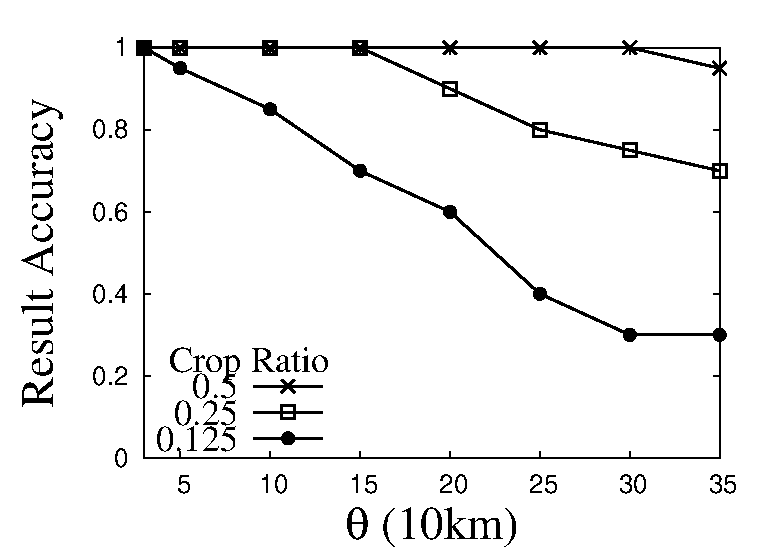
\epsfig{file=mparameter.eps,width=0.8\columnwidth}
%\caption{Performance Under Different Distortion}
%\label{fig:m}
%\end{figure}

%\begin{figure}[h]
%\centering
%\epsfig{file=mdelta.eps,width=0.6\columnwidth}
%\caption{Distortion Added by Watermarking}
%\label{fig:dis}
%\end{figure}

\begin{figure}[h]
\centering
\subfigure[Distortion]{
  \label{fig:dis}
  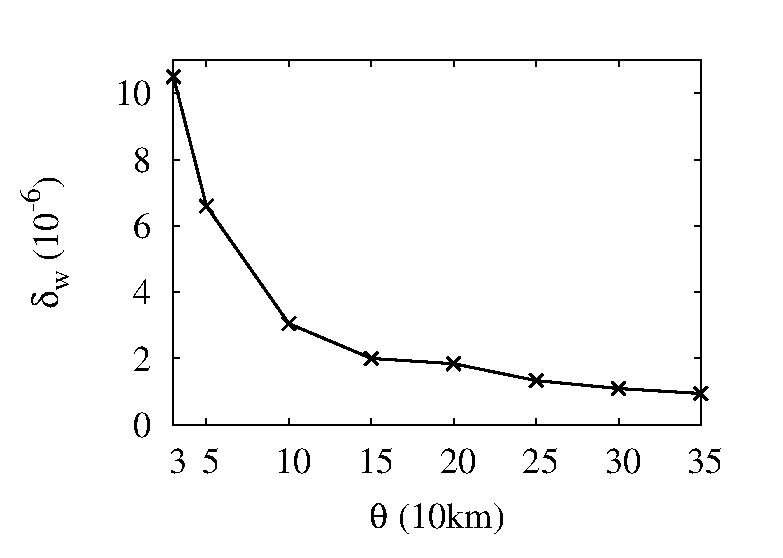
\epsfig{file=images/mdelta.eps,width=0.45\columnwidth}
}
\subfigure[Different Crop Ratio]{
  \label{fig:m}
  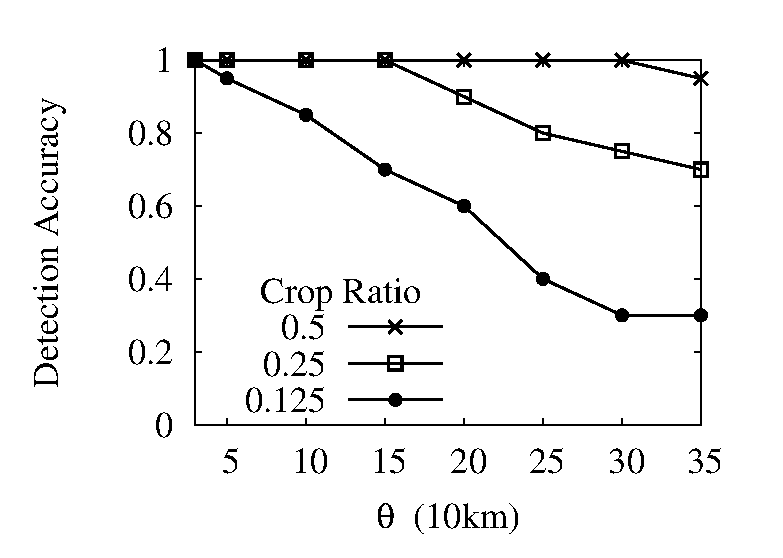
\epsfig{file=images/mparameter.eps,width=0.45\columnwidth}
}
\subfigure[Time of Insertion]{
  \label{fig:ti}
  \epsfig{file=images/time.eps,width=0.45\columnwidth}
}
\subfigure[Time of Detection]{
  \label{fig:td}
  \epsfig{file=images/time1.eps,width=0.45\columnwidth}
}
\caption{Experiment Results under Different Distortion}
\label{fig:pudd}
\end{figure}

%\begin{table}[th]
%\centering
%\caption{Distortion Added by Watermarking}
%\label{tab:dis}
%\begin{tabular}{|c||c|c|c|c|c|c|c|c|} 
%\hline
%$\theta$(km) & 3 & 5 & 10 & 15 & 20 & 25 & 30 & 35 \\\hline \hline
%$\delta (10^{-6})$ & 10.50 & 6.60 & 3.05 & 2.00 & 1.84 & 1.33 & 1.09 & 0.94 \\\hline
%\end{tabular}
%\end{table}

In the following experiment, we watermark a map with certain distortion, here we set 
$\theta =30,000$. After that we crop different ratio from the map to evaluate the performance 
of our algorithm. For each crop ratio, we select different parts of the map to detect 
up to 20 times. We randomly select different parts of the watermarked map to detect (see 
Figure \ref{fig:cropmethod}) and calculate the detection accuracy. Here we also implement 
Voigt's and Pu's methods to make a comparison. Distortion $\delta_w$ added by the watermarking 
is $10.5\times 10^{ -6 }$ (Jiang), $10.8\times 10^{-6}$ (Voigt) and $9.8\times 10^{-6}$ (Pu). 
The distortion of all three methods are almost at the same level.
Figure \ref{fig:cropattack} gives the results.

%\begin{figure}[th]
%\centering
%\subfigure[Time of Insertion]{
%  \label{fig:ti}
%  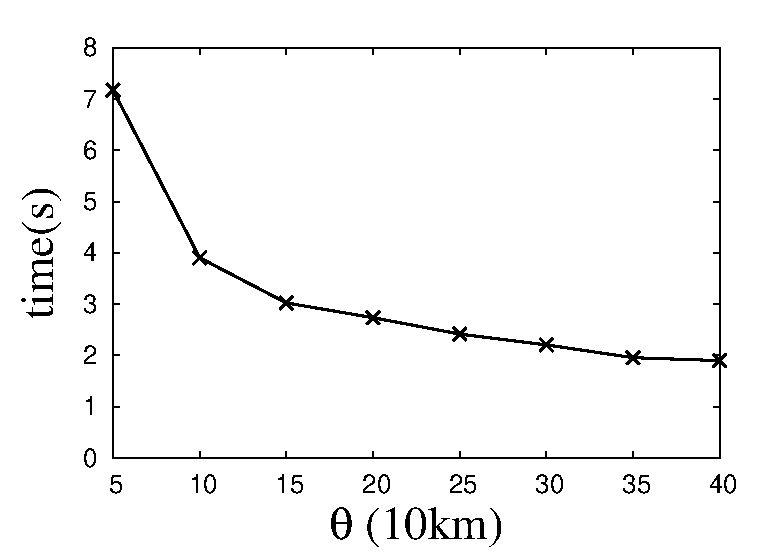
\epsfig{file=time.eps,width=0.45\columnwidth}
%}
%\subfigure[Time of Detection]{
%  \label{fig:td}
%  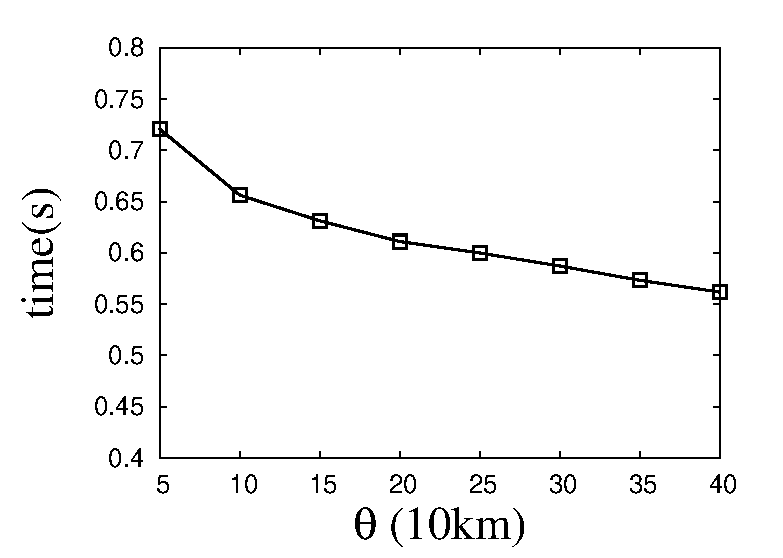
\epsfig{file=time1.eps,width=0.45\columnwidth}
%}
%\caption{Experimental Time Results}
%\label{fig:results}
%\end{figure}

%\begin{figure}[th]
%\centering
%\epsfig{file=cropattack.eps,width=0.7\columnwidth}
%\caption{Performance Under Different Crop Ratio}
%\label{fig:cropattack}
%\end{figure}

\begin{figure}[h]
\centering
\subfigure[\scriptsize Performance under Cropping]{
  \label{fig:cropattack}
  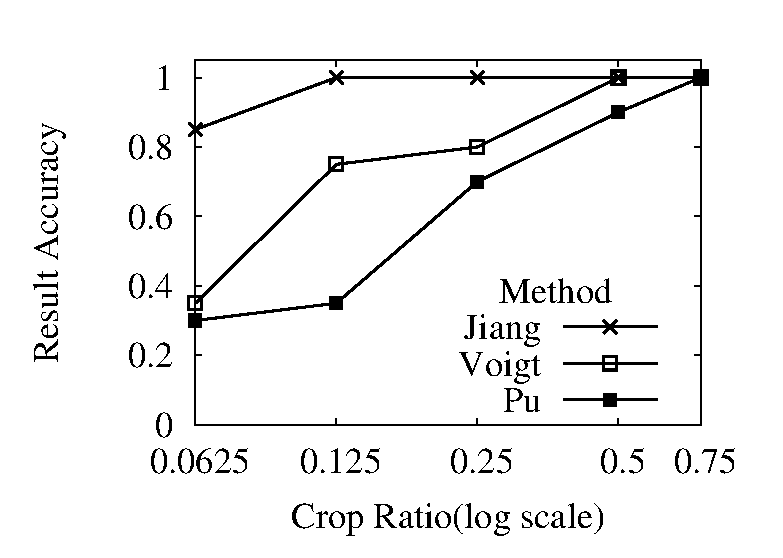
\epsfig{file=images/cropattack.eps,width=0.47\columnwidth}
}
\subfigure[\scriptsize Accuracy in $1/8$ crop ratio]{
  \label{fig:mdelta}
  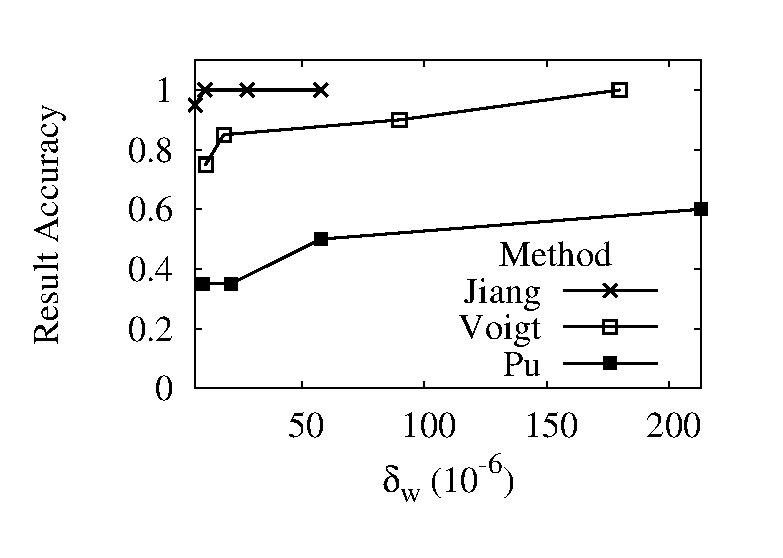
\epsfig{file=images/delta.eps,width=0.47\columnwidth}
}
\caption{Performance under Crop Attack}
\end{figure}

According to the experiment result, we can find that our algorithm keeps a perfect
result when the crop ratio is up to $1/8$, while the comparison methods show a significant
accuracy degradation. And when crop ratio is $1/16$, we still contain a high accuracy.
We also test the detection accuracy under different distortion in $1/8$ crop ratio
(see Figure \ref{fig:mdelta}). In this experiment, our algorithm can attain
a $100\%$ detection accuracy with just little distortion. Since the detection accuracy of 
our algorithm quickly attain to $1$, it is not necessary to plot too many points in Figure 
\ref{fig:mdelta}.

%\begin{figure}[h]
%\centering
%\epsfig{file=delta.eps,width=0.7\columnwidth}
%\caption{Detection Accuracy in $1/8$ crop ratio}
%\label{fig:mdelta}
%\end{figure}

\subsection{Performance under Merge Attack}
%\JK{For merge part, I plan to design two experiments:\\
%1).I plan to watermark a map with the same distortion distance as crop 3) and 
%make a merge map like figure \ref{fig:merge}. What I want to show the readers is
%a direct result of the merge detection result: suspicious regions and detection
%confidence. A visual figure can also be drawn.\\
%2).Just like merge 3), I plan to crop the watermarked map into different ratio
%and merge with the other data source to make different maps, for each ratio, 20
%different merge maps will be detected. The result will be a ``Detection accuracy-
%watermarked ratio''figure for all three algorithms.} 

%\KZ{So (1) is a special case of (2) which is actually fig 15 right? For
%(1) you will just have a detection number for 3 algorithms? I think you can
%show visually what was the original merge situation and what was the 
%portion that you detected by comparing and contrasting the difference in
%a figure. That will be visually impactful.}

In this experiment, we select the $2012$ TIGER map of Minneapolis-St. Paul 
Metropolitan area as another data source, which can be downloaded from the 
United States Census Website\cite{tigerurl}. The coordinate system of TIGER 
map is different from MN dot base Map. We transform the coordinate system of 
TIGER map to make it same as the former data source. Figure \ref{fig:17} is 
the overlap of these two maps of Anoka county after the synchronization. 
%As we can see that very slight difference could be found between these two maps, 
%so we have a good reason to believe that if we implement our partition algorithm 
%on a merge map of them, the result will almost be the same.


\begin{figure}[th]
\centering
\epsfig{file=images/overlap.eps,width=0.7\columnwidth}
\caption{Overlap of Two Maps}
\label{fig:17}
\end{figure}
We crop a watermarked map ($\delta_w = 6.60 \times 10^{-6}$) and merge part of it with TIGER 
map to make a ``new'' map (see Figure \ref{fig:mattack}). The result of the 
merge detection: suspicious regions and detection confidence is shown in Table 
\ref{tab:merge}. Here we select those regions which have at least 10 points tested. 
From the corresponding visual figure (see Figure \ref{fig:mresult}), we can see 
that our algorithm almost ``exactly'' decides the suspicious regions. 

\begin{figure}[h]
\centering
\subfigure[\scriptsize Merge Attack]{
  \label{fig:mattack}
  \epsfig{file=images/mattack.eps,width=0.42\columnwidth}
}
\subfigure[\scriptsize Detection Result]{
  \label{fig:mresult}
  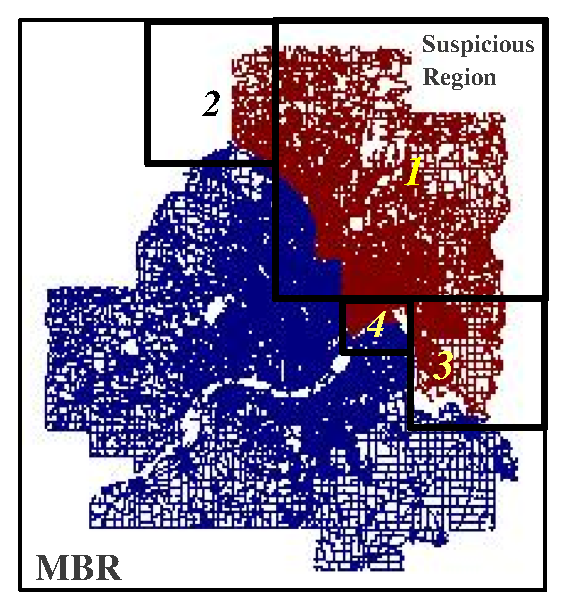
\epsfig{file=images/mresult.eps,width=0.42\columnwidth}
}
\caption{Merged Map}
\end{figure}

%\begin{figure}[th]
%\centering
%\epsfig{file=merge.eps,width=0.8\columnwidth}
%\caption{Merged Map}
%\label{fig:mergeexp1}
%\end{figure}


\begin{table}[th]
\centering
\caption{Merge Attack Detection}
\label{tab:merge}
\begin{tabular}{|c||c|c|c|c|} 
\hline
Region & Total & Match & Confidence & Result \\\hline \hline
1 & 147 & 122 & 1.000 & positive\\\hline
2 & 12 & 11 & 0.997 & positive\\\hline
3 & 23 & 18 & 0.994 & positive\\\hline
4 & 15 & 12 & 0.983 & positive\\\hline
\end{tabular}
\end{table}

We also watermark the Minneapolis-St. Paul Metropolitan area and then split this 
watermarked map into the same small portions as cropping experiment above. After 
that we merge these maps with the complementary parts of map from TIGER to create 
some new digital road maps. In this experiment, we also implement the two other 
method to make a comparison. Distortion $\delta_w$ added by the watermarking still
is $10.5\times 10^{ -6 }$ (Jiang), $10.8\times 10^{-6}$ (Voigt) and $9.8\times 10^{-6}$ (Pu). 
Figure \ref{fig:mergeattack} shows the result of our 
experiments.

%\begin{figure}[th]
%\centering
%\epsfig{file=mergeattack.eps,width=0.7\columnwidth}
%\caption{Performance Under Merge Attack}
%\label{fig:mergeattack}
%\end{figure}

\begin{figure}[h]
\centering
\subfigure[\scriptsize Performance under merging]{
  \label{fig:mergeattack}
  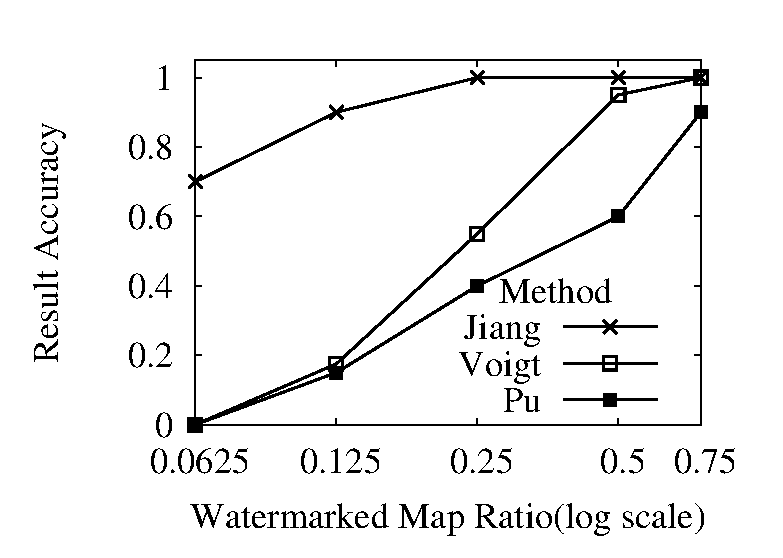
\epsfig{file=images/mergeattack.eps,width=0.47\columnwidth}
}
\subfigure[\scriptsize Accuracy in $1/8$ merge ratio]{
  \label{fig:deltamerge}
  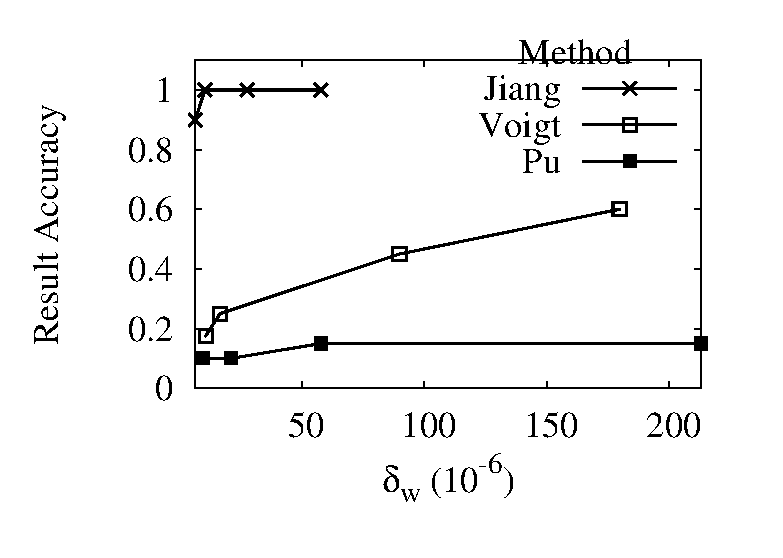
\epsfig{file=images/deltamerge.eps,width=0.47\columnwidth}
}
\caption{Performance under Merge Attack}
\end{figure}

Comparing with the cropping experiment, we can obviously find the performance of 
our proposed algorithm is almost not affected by the complementary part of the map. 
However, the detection accuracy of the other two methods decrease significantly. 
The reason is the complementary map provides sufficient disturb to watermarked data.
Similarly, we also implement another experiment to evaluate the relationship between
detection accuracy and watermark distortion $\delta_w$. From this figure, we can see that
our algorithm still can quickly attain a quite high detection accuracy. However, when 
$\delta_w$ increases for Pu's and Voigt's method, the detection accuracy doesn't changed significantly.
The reason for Pu should be that it's global liner correlation is destroyed by ``merge'' attack.
For Voigt's method, though more watermark information is used for detection, more ``merge'' 
noise will will also be added to the detection process. Thus increase of detection accuracy
for them is not significant.



%\begin{figure}[h]
%\centering
%\epsfig{file=deltamerge.eps,width=0.7\columnwidth}
%\caption{Detection Accuracy in $1/8$ Merge ratio}
%\label{fig:deltamerge}
%\end{figure}



%%% Local Variables:
%%% mode: latex
%%% TeX-master: "paper"
%%% End:

\section{RELATED WORK}
\label{sec:related}
%\KZ{Divide all the papers into a few categories or types, discuss them separately,
%then summary the work within a category with its pros and cons and compare with
%our work. More focus should be given to the two methods that we compared with in
%the evaluation.}
Many efforts have been made to protect the copyrights of 
multimedia products such as images, movies and music. 
% \cite{BoneyTH96,ChangA01}. 
%Watermarking techniques, 
%which helps the IP owner to declare the rightful ownership of a product, 
%have attracted researchers' interests. 
%Multimedia data usually includes redundant information with respect to 
%the human perceptual system. Thus, much bandwidth is available in these 
%datasets to hide small pieces of extra information, or watermarks. 
%A wide variety of watermarking techniques 
%have since been developed in many of domains. 
Digital road maps is a special vector graphics data which contains important
geographical and spatial information. In the rest of this section, we will
focus on GIS spatial data watermarking but will also briefly touch on related
techniques in some other domains.
The technique proposed in this paper benefits from or is inspired 
by some of these methods.

\subsection{GIS Spatial Data Watermarking}
Several studies have touched on the watermarking of GIS spatial data such as digital 
vector maps. Even though digital vector maps are represented by node coordinates which 
can also be treated as relational tables, techniques developed for relational data 
ignore the spatial properties of road maps such as spatial distances and geo-localities.
These distinct features of GIS spatial data call for special treatments in watermarking
techniques. According to Niu \cite{Niu06:Survey}, the existing methods of 
digital vector map watermarking is classified into two categories: 
algorithms in spatial domain and algorithms in frequency domain. 
Depending on whether to require the original map 
for detection, these methods are also classified as the not blind and the blind.
In addition, algorithms can also be categorized into {\em global} or {\em local}
depending on whether global information of the map is needed when computing each
watermark.

The spatial domain algorithms embed watermarks based on the geometric properties of 
polyline and polygon objects. It is often easier to control the amount of distortion
added by the watermarks. They are also more robust against rotation, scaling 
and noises, while preserving the utility of a map. 
Existing methods in spatial domain usually lack of robustness against massive cropping and merging. 
%\KZ{I don't really understand the above sentence. Please elaborate. Also say
%how our method avoided these drawbacks.}
The method proposed in this paper falls into the category of spatial domain algorithms. 

The frequency domain algorithms essentially transform the original data into
frequency domain, usually by Discrete Fourier Transform (DFT) 
\cite{Kitamura01:DFT,DFT,Illustration} or Discrete Wavelet Transform (DWT)
\cite{Liyuanyuan03}, add noises in the frequency domain and then transform it
back into the spatial domain.  
The critical drawbacks of frequency domain techniques are the 
difficulty of controlling the amount of distortion in the spatial domain
and the lack of robustness against data cropping and data reordering, due to
the fact that it is actually a global watermarking scheme. 
 %\KZ{Check the above to see if it's correct. Also we didn't mention
%local algorithms. Maybe mention a bit here also?} 

\subsubsection{Non-Blind Methods in Spatial Domain}
Some watermarking methods \cite{Han06:Adaptive,OhbuchiUE02,OhbuchiUE03} 
require the original map or watermarked map as a reference to detect watermarks 
from a suspicious map. This kind of methods are called ``non-blind'' algorithms.
The main weakness of these methods is that road maps can be updated over time
and a map producer may have many versions of the same map in its database.
Moreover in the same database, there could be many maps which have overlapping
regions, say map of the Twin Cities, map of Minnesota, map of the United States, etc.
When the map database is big, and when the suspicious map could have been
subjected to cropping and merging, it is not easy to identify the original map.
%which are not realistic because it is very time-consuming to find 
%a corresponding digital map from a map database.
%An improved adaptive watermarking algorithm\cite{Han06:Adaptive} subdivides the map into some 
%uniform size rectangular blocks and insert the watermark into each block. Before extraction,
%it does not compare the the watermarked map with the primitive map, but the original 
%watermarked map. This is not a blind watermarking algorithm. 

Ohbuchi et al.\cite{OhbuchiUE02} partitions the space of the digital map 
into rectangles such that every rectangle contains almost equal node numbers. 
Then the $v^{th}$ vertex inside 
the rectangle is modified to include a watermark. In another method \cite{OhbuchiUE03}, 
all vertices are connected into a single mesh by Delaunay triangulation. 
Then a mesh Laplacian is formed and the mesh is partitioned into patches using 
the same method as in the former one\cite{OhbuchiUE02}. 
Mesh-spectral coefficients are calculated for every patch and the watermark is embedded into 
these coefficients. 
%\KZ{rephrase the above sentence.} 

Both of the above algorithms disperse watermarks locally and have 
some robustness against crop attack. 
However, them are highly dependent on the validity of the original data. 
When extracting the watermark, the suspicious map is aligned onto the original map. 
All inserted nodes have to be deleted, and all removed nodes have to be correctly 
recovered.

\subsubsection{Blind Methods in Spatial Domain}
Some other watermark framework are proposed which required no original or watermarked map
as a reference. Some of these methods \cite{Huo10:Polyline,KangKC01,YanLW11,Spr:scheme} 
insert watermark globally. 
%The work by S. Khanna \cite{KhannaZ00} watermarks 
%digital road maps by altering the shortest path with smallest node numbers. 
%The assumption is that the shortest path will not be affected by attacks. 
%\KZ{Shortest path between which two points?}
Yan et al. proposed a key point based algorithm \cite{YanLW11}. 
Key points are those nodes in the map which have more important geometric aspects 
than the other ones, for example cross joints and those in sharp curve. 
They are not likely to be removed or edited by the attackers because removing them
will render the map useless.  This method uses a dynamic programming 
algorithm \cite{DOUGLASD.H.:1973} both in insertion and detection steps. 
Key points in the map are used for inserting and detecting watermarks. 
This kind of algorithms are robust against some attacks like noise and vertex simplification, 
but are still vulnerable to crop and merge attacks.  %\KZ{If it's a local algorithm, why can't it
%detect the remaining watermarks?} 
% \KZ{Don't understand the above method.}

%The scheme for polyline \cite{Huo10:Polyline} 
%proposed an algorithm to calculate the length and perimeter of the polylines and polygons in 
%a map and cluster polylines polygons to some group with the uniform step of length and 
%perimeter dynamic range. And embed the watermark bit to local mean of lengh/perimeter of 
%polylines/polygons in a suitable group. Then embed the watermark bit to the points coordinates. 
%In this approach, the group is clustered by length/perimeter of the objects and these objects 
%is probability located in any position of the map. 

Other blind watermarking algorithms
\cite{Voigt:2003,Schulz:2004,PuDJ06,Bird09:Shape,Kim11:copyright} 
provide some limited resistance against crop attacks to some extent. 
Voigt et al.\cite{Voigt:2003} 
proposed a feature based watermarking algorithm which is relies on statistical detection. 
This method partitions a map into small rectangular regions called ``patches''. 
It then randomly selects two subsets of the patches called set $A$ and set $B$,
respectively. Next, it calculates a reference point for each patch in the two set.
During watermark insertion, all nodes in set $A$ are shifted {\em toward} the reference point
in their respective patches, while all nodes in set $B$ are shifted {\em away} from
the reference point. The amount of shift is governed by an $F$-distribution 
\cite{abramowitz1965handbook}
%\KZ{Give a citation here cos not everybody knows what it is.}
which is also used to detect the watermark.
%ware relative coordinates against the bottom-left corner of each patch.
%For each set, it computes a relative reference point
%inside the patches to a relative value w.r.t. some original vertices inside the patches. 
%During insertion of watermarks, the distance of vertice to a 
%reference line in one patch list is increased while the distance to the line in
%the other patch list decreased. The ratio of standard error of point
%coordinates in two patch list follows a $F$ distribution, 
%which is used to decide whether the map is watermarked. 
%This algorithm is robust against several attacks, including cropping to some extent.  
%Another high capacity robust 
%scheme\cite{Schulz:2004} is also proposed . They divide the original map into many vertical 
%or horizontal strips with a certain width. The vertices belonging to each strip are shifted 
%to special locations to represent bit 1 or 0. The scheme has the robustness to additional 
%noises within tolerance and map shifting, and to some extent map cropping. However, this 
%method almost changed all points of a map, which will introduce too much distortion.
Pu et al. proposed a blind algorithm \cite{PuDJ06} which 
divides the map into mesh segments, and then
embeds the watermark in each segment with a fixed order. 
In the detection step, each segment is evaluated by a correlation parameter, which
is a linear correlation of the watermark and the watermarked data. 
%\KZ{Elaborate a bit on the correlation param?}
To survive crop attack, a global correlation based detection method is 
applied as an optimization. This algorithm watermarks maps according to 
their topological relations. 

While these algorithms present some resistance against cropping attack, 
they cannot survive cropping at larger scale.
Take Voigt\cite{Voigt:2003} as an example, when the watermarked map is 
massively cropped, many patches that are marked may be
removed. Thus $F$ distribution of watermarked points may be destroyed. 
Therefore, the method is not robust enough against ``massive crop''. 
%\KZ{Above is repetition of the earlier discussion but it's
%still not clear why removing ``patches'' causes the algo to fail.} 
Furthermore, if the map is cropped and then merged with others, 
the information added by the merge will defeat the watermarking more easily.

\subsubsection{Methods in Frequency Domain}
 
Solachidis et al.\cite{DFT} proposed a blind watermarking scheme embedding 
a single bit into a polyline by modifying the discrete Fourier coefficients 
of polyline's coordinate sequence.  This method embeds the watermark in 
the magnitude of the curve's Fourier descriptors to exploit 
its location, scale, and rotation invariant properties. Due to the amplitude frequency 
features of discrete Fourier transform, the algorithm is inherently robust to many attacks 
such as map translation, rotation, scaling and changing start vertex. Similar to the DFT 
method\cite{DFT}, Li et al. proposed a blind scheme \cite{Liyuanyuan03} embedding 
multi-bits into a vector map in DWT domain. 
These frequency domain methods rely on the integrity
of map and order of data points. When part of map data is removed or the order 
of data points is changed, the coefficients will 
also be changed, which makes them extremely vulnerable to crop 
and merge attacks.
%\KZ{Don't understand the above sentence, rephrase?}


\subsection{Watermarking in Other Domains}
%Watermarking techniques are widely used to protect the copyrights of media 
%such as image, video, and audio data . 
%Because of their success in protecting multimedia data, 
%watermarking techniques have been extended to other
%fields. Text/Language watermarking has only low bandwidth to include watermark 
%and at the same time must provide acceptable level of resilience to different attacks. 
%A natural language watermarking technique \cite{NLW} inserts watermarking by 
%constructing a text meaning representation tree.

Some research attention has been given to relational data\cite{AgrawalK02,SionAP03}. 
Rakesh Agrawal proposes a framework of watermarking relational databases\cite{AgrawalK02}. 
According to this approach, a primary key is stored in some significant 
tuples of relational data. The altered attribute index and bit 
index for the selected attribute are randomly 
selected according to secret keys. Their approach is highly dependent on the primary key 
of the data tuple and randomly selects a subset of tuples to watermark. This approach in 
fact disperses one bit watermark into different position of relational data. It provide 
some resistance against crop and merge attack to some extent. 
Some ideas in this framework actually inspired the work in this paper, e.g.,
modifying least significant bits and computing the confidence of detection.
However, this framework is for relational data and hence does not consider 
the special properties of spatial attributes in GIS spatial data. In our method,
information which is adjacent to each other in geographical space collaborate to
decide the watermarking positions. However, in relational data, different tuples
are completely independent to each other, even though they are stored together,
because they form a set.
%\KZ{You discussed many details of the above algo but not enough discussion
%about the connection with our method, most importantly the key differences
%between the two (other than that it was for relation data. Any other
%differences?}
Other work\cite{SionAP03} extends the framework\cite{SionAP02} 
to relational databases. In that paper, numeric dataset are first hashed 
to another dataset with a secret order.  Then the new dataset is grouped 
into different chunks according to their order. 
Finally, the average value and standard deviation is calculated for every chunk. 
According to these statistics and watermarking data, 
a small number of data points are altered. 
This approach still disperses the watermark globally. 
One of the serious drawbacks for this global watermarking approach is that 
it completely fails a "massive crop" attack.


%\section{Future Work}
%%To this end, we have successfully built a system
%%which can solve the top-$k$ extraction problem
%%with adequate accuracy and efficiency.
%%With the big data experiment result,
%%we have built a top-$k$ database with
%%over 1.7 million top-$k$ lists of 92.0\% precision.
%%In the future, we will mainly focus on three aspects of work.
%
%The first One is to further enrich the top-$k$ database
%and improve its quality. On the one hand,
%we can use larger training data and
%more sophisticated machine learning models to
%upgrade the system performance;
%on the other hand, we can explore the other source
%of top-$k$ lists rather than top-$k$ pages.
%The slide-show pages can be a good candidate (e.g. Fig. \ref{fig:slideshow}),
%as the top-$k$ list spans across a set of pages, which are connected one another
%by hyperlinks. Intuitively, we can develop a crawler that goes through
%``Previous'' and ``Next'' links and obtain a slide-show page chain.
%But the main challenge is we can not run it on big data as the web snapshot
%cannot support random access (access by URL).
%Furthermore, the snapshot may lose some nodes in a page chain,
%thus we cannot extract the complete list.
%
%The second is to further understand top-$k$ lists, especially the top-$k$ titles.
%In Section \ref{sec:problem}, we define a function $tr$ to convert a textual title
%into a five-tuple representation, which is implemented by Title Classifier.
%However, this representation remains rough as we miss some modifiers other than time and location.
%For example, ``top 10 NBA players alive'' is different from ``top 10 NBA players who have a ring'',
%but they will share the same representation. We may need to include those modifiers in the representation,
%and redefine $tr$ as $tr : (t, d) \rightarrow \mathcal{R} = (k, c, \alpha,
%\mathcal{M})$ where $\mathcal{M}$ is a set of modifiers including the temporal modifier $\tau$ and
%spatial modifier $\sigma$. To do this, we need to improve our Title Classifier to recognize general modifiers,
%probably using the same technology.
%A harder challenge is to calculate semantical similarity between $\mathcal{R}$.
%%which can be defined as $sim : (\mathcal{R_1}, \mathcal{R_2}) \rightarrow score$.
%To solve this, we need to find out the similarity of each part
%($sim_c(c_1, c_2)$, $sim_\alpha(\alpha_1, \alpha_2)$ and $sim_\mathcal{M}(\mathcal{M}_1, \mathcal{M}_2)$)
%and develop a equation/model $sim : (sim_c, sim_\alpha, sim_\mathcal{M}) \rightarrow score$.
%With this function, we can cluster the top-$k$ lists into groups of similar semantics.
%
%The last is to utilize the top-$k$ database.
%As we discuss in Section \ref{sec:intro},
%we attempt to build a Q/A system.
%%which,
%%according to different type of queries,
%%return an instance (e.g. ``Who is the second tallest building in Beijing'') or
%%a ranked list (e.g. ``top 10 richest people in 2010'').
%Given a query $q$, we can first parse it into the tuple representation $\mathcal{R}_q=(k_q,...)$ and
%find a most similar group $g$ from the database.
%To generate a $k_q$-items ranked list (or the $k_q$th item) from $g$, there are two possible solutions.
%The list-wise approach is to (1) rank the lists in $g$ which contain more than $k_q$ items,
%and (2) return the first $k_q$ items (or the $k_q$th item) of the best list.
%The item-wise approach is to merge top-$k$ lists in a group into a bigger one,
%where the main challenge is to calculate the ranking score of each item over aggregation (of ranked lists)
%as an item can exists in multiple top-$k$ lists with different position(ranking within the list).
%This problem is popular in the area of top-$k$ query processing
%as some algorithms are proposed to solve it in different scenarios
%\cite{angel2009ranking,chakrabarti2006ranking,bansal2008ad}.
%In general, we need
%
%
%To obtain the ranking score of each item $i$,
%we need to calculate the score $s_i$ wrt. each list $L_i$ that contains $i$
%(which should be a function of item position $p_i$ and the list size $|L_i|$).
%
%
%We can first define a function $rp: (k, n) \rightarrow score$,
%which gives the score of the $n$th item in any top-$k$ list.
%Then for a instance $i$, assuming it
%
%
%%.
%%The main challenge is to calculate the ranking of each item over aggregation of lists,
%%while a similar problem in the area of top-$k$ query processing
%
%For a list item $i$, it may appears in different list $L$
%The final solution may be a hybrid of the two approach above.



\section{Conclusion}
\label{sec:conclusion}
This paper presents a novel and interesting problem of extracting
top-$k$ lists from the web.  Compared to other structured data,
top-$k$ lists are cleaner, easier to understand and more
interesting for human consumption, and therefore are an important
source for data mining and knowledge discovery. We demonstrate a
algorithm that automatically extracts over 1.7 million such lists from
the a web snapshot and also discovers the structure of each list.  Our
evaluation results show that the algorithm achieves 92.0\% precision
and 72.3\% recall.

%\ZZX{
%In the future, we will focus on building a Q/A system based on
%the large number of top-$k$ lists we extracted.
%%According to different type of queries,
%%the system should return
%%a $k$-item ranked list or the $k$th instance, where $k$ is specified in the query.
%As a top-$k$ query processing system, 
%the main challenge lies in how to generate a $k$-item ranked list 
%from all top-$k$ lists that matches the query.
%Basically we can return the first $k$ items from the best-matching list 
%that contains more than $k$ items.
%A more complicated approach is to merge top-$k$ lists in a group into a bigger one,
%where we need to calculate the ranking score of each item over aggregation (of ranked lists)
%\cite{fagin2001optimal,angel2009ranking,chakrabarti2006ranking}.
%The final solution may be a hybrid of the two approaches above.
%}
%
%Ideally, we should first cluster the top-$k$ lists into groups of similar semantics
%and find out the group $g$ that match the query best.
%To generate a $k$-items ranked list (or the $k$th item) from the group, there are two possible solutions.
%The list-wise approach is to rank the lists in $g$ which contain more than $k$ items,
%and return the first $k$ items (or the $k$th item) of the best list.
%The item-wise approach is to merge top-$k$ lists in a group into a bigger one,
%where is to calculate the ranking score of each item over aggregation (of ranked lists)
%\cite{angel2009ranking,chakrabarti2006ranking,bansal2008ad}.
%The final solution may be a hybrid of the two approaches above.
%}
%
%The format of query is similar to a top-$k$ title,
%which can be represent as a 5-tuple as well
%(e.g. ``Who is the second tallest building in Beijing'' can be represent as (2, building, tallest, in Beijing, none)).
%And the system should return a $k$-item ranked list (or the $k$th item) as answer.
%There are two possible solutions.
%The list-wise approach is to find a best-fitting top-$k$ list according to the query,
%that contains no less than $k$ items.
%The item-wise approach is to cluster the top-$k$ lists into groups of similar semantics.
%and aggregate top-$k$ lists in a group into a bigger ranked list.
%Then given a query, we can find the best-fitting group and return the first $k$ items in the bigger list.
%The final solution may be a hybrid of the two approach above.

%According to different type of queries,
%the system should return an instance (e.g. ``Who is the second tallest building in Beijing'') or
%a ranked list (e.g. ``top 10 richest people in 2010'').
%There are two possible solutions.
%The list-wise approach


%\bibliographystyle{abbrv}
%\renewcommand{\baselinestretch}{0.9}
%\bibliography{watermark}
% watermark.bib is the name of the Bibliography in this case
\begin{thebibliography}{10}

\bibitem{mndoturl}
{MN}/{DOT}.
\newblock \url{http://www.dot.state.mn.us/}.

\bibitem{tigerurl}
{TIGER}.
\newblock \url{http://www.census.gov/}.

\bibitem{abramowitz1965handbook}
M.~Abramowitz and I.~Stegun.
\newblock {\em Handbook of mathematical functions: with formulas, graphs, and
  mathematical tables}, volume~55.
\newblock Dover publications, 1965.

\bibitem{AgrawalK02}
R.~Agrawal and J.~Kiernan.
\newblock Watermarking relational databases.
\newblock In {\em VLDB}, pages 155--166, 2002.

\bibitem{Bird09:Shape}
S.~Bird, C.~Bellman, and R.~v. Schyndel.
\newblock A shape-based vector watermark for digital mapping.
\newblock In {\em Proceedings of the 2009 Digital Image Computing: Techniques
  and Applications}, pages 454--461. IEEE Computer Society, 2009.

\bibitem{DOUGLASD.H.:1973}
D.~H. Douglas.
\newblock Algorithms for the reduction of the number of points required to
  represent a line or its a caricature.
\newblock {\em The Canadian Cartographer}, 10(2):112--122, 1973.

\bibitem{Han06:Adaptive}
P.~Han, J.~Gong, and L.~Cheng.
\newblock An improved adaptive watermarking algorithm for vector digital maps.
\newblock In {\em Geoscience and Remote Sensing Symposium,IGARSS}, pages 2844
  --2847, 2006.

\bibitem{Huo10:Polyline}
X.-J. Huo, T.-Y. Seung, B.-J. Jang, S.-H. Lee, and K.-R. Kwon.
\newblock A watermarking scheme using polyline and polygon characteristic of
  shapefile.
\newblock In {\em ICINIS, 2010}, pages 649 --652, 2010.
\vfill\eject
\bibitem{GangKC01:mask}
H.~Kang, K.~Kim, and J.~Choi.
\newblock A vector watermarking using the generalized square mask.
\newblock In {\em ITCC}, pages 234--236. IEEE Computer Society, 2001.

\bibitem{Kim11:copyright}
J.~Kim, S.~Won, W.~Zeng, and S.~Park.
\newblock Copyright protection of vector map using digital watermarking in the
  spatial domain.
\newblock In {\em Digital Content, Multimedia Technology and its Applications
  (IDCTA), 2011 7th International Conference on}, pages 154 --159, aug. 2011.

\bibitem{Kitamura01:DFT}
I.~Kitamura, S.~Kanai, and T.~Kishinami.
\newblock Copyright protection of vector map using digital watermarking method
  based on discrete fourier transform.
\newblock In {\em Geoscience and Remote Sensing Symposium, 2001. IGARSS '01.
  IEEE 2001 International}, volume~3, pages 1191 --1193 vol.3, 2001.

\bibitem{Spr:scheme}
S.-H. Lee and K.-R. Kwon.
\newblock Vector watermarking scheme for {GIS} vector map management.
\newblock {\em DOI10.1007/s11042-011-0894-y SpringerLink}, 2011.

\bibitem{Liyuanyuan03}
Y.~Li and L.~Xu.
\newblock A blind watermarking of vector graphics images.
\newblock In {\em ICCIMA '03: Proceedings of the 5th International Conference
  on Computational Intelligence and Multimedia Applications}, page 424,
  Washington, DC, USA, 2003. IEEE Computer Society.

\bibitem{Niu06:Survey}
X.~Niu, C.~Shao, and X.~Wang.
\newblock A survey of digital vector map watermarking.
\newblock In {\em 2006 International Journal of Innovative
  Computing,Information and Control Volume 2}, 2006.

\bibitem{OhbuchiUE02}
R.~Ohbuchi, H.~Ueda, and S.~Endoh.
\newblock Robust watermarking of vector digital maps.
\newblock In {\em ICME (1)}, pages 577--580, 2002.

\bibitem{OhbuchiUE03}
R.~Ohbuchi, H.~Ueda, and S.~Endoh.
\newblock Watermarking 2d vector maps in the mesh-spectral domain.
\newblock In {\em Shape Modeling International}, pages 216--228, 2003.

\bibitem{PuDJ06}
Y.-C. Pu, W.-C. Du, and I.-C. Jou.
\newblock Toward blind robust watermarking of vector maps.
\newblock In {\em ICPR (3)}, pages 930--933, 2006.

\bibitem{Schulz:2004}
G.~Schulz and M.~Voigt.
\newblock A high capacity watermarking system for digital maps.
\newblock In {\em MM{\&}Sec}, pages 180--186, 2004.

\bibitem{SionAP02}
R.~Sion, M.~J. Atallah, and S.~Prabhakar.
\newblock On watermarking numeric sets.
\newblock In {\em IWDW}, pages 130--146, 2002.

\bibitem{SionAP03}
R.~Sion, M.~J. Atallah, and S.~Prabhakar.
\newblock Rights protection for relational data.
\newblock In {\em SIGMOD Conference}, pages 98--109, 2003.

\bibitem{DFT}
V.~Solachidis and I.~Pitas.
\newblock Watermarking polygonal lines using fourier descriptors.
\newblock {\em Computer Graphics and Applications, IEEE}, 24(3):44 -- 51,
  may-jun 2004.

\bibitem{Illustration}
H.~Sonnet, T.~Isenberg, J.~Dittmann, and T.~Strothotte.
\newblock Illustration watermarks for vector graphics.
\newblock {\em Computer Graphics and Applications, Pacific Conference on},
  0:73, 2003.

\bibitem{Voigt:2003}
M.~Voigt and C.~Busch.
\newblock Feature-based watermarking of 2d-vector data.
\newblock In {\em SPIE,Security and Watermarking of Multimedia Content.Santa
  Clara,}, pages 359--366, 2003.

\bibitem{YanLW11}
H.~Yan, J.~Li, and H.~Wen.
\newblock A key points-based blind watermarking approach for vector geo-spatial
  data.
\newblock {\em Computers, Environment and Urban Systems}, 35(6):485--492, 2011.

\end{thebibliography}
\end{document}
